\documentclass[a4paper,10pt,twoside]{article}
\usepackage[left=2cm,right=2cm,top=3cm,bottom=2cm,includeheadfoot]{geometry}
\usepackage{textcomp}

\usepackage{fancyhdr}
\usepackage[pdftex]{graphicx}
\usepackage{amssymb}
\usepackage{hyperref}
\usepackage{amsmath}
\usepackage{amsthm}
\newtheorem{myTheorem}{Theorem}
\newcommand{\lien}[1]{\href{#1}{\nolinkurl{#1}}}
\usepackage[pdftex]{graphicx,color}  
% ------------------- Definitions -------------------
\def \TITLE{Efficient convolution using the Fast Fourier Transform,\\ Application in C++}
\def \SUBTITLE{Convolution product and Fast Fourier Transform}
\def \AUTHOR{Jeremy Fix}

\newcommand{\M}[1]{$\mathrm{#1}$}
\newcommand{\HEADING}[1]{\vspace{1pt}\paragraph*{#1}\ \\}

% -------------------   Document   -------------------
\begin{document}
\sffamily 
\renewcommand{\familydefault}{\sfdefault}

% Page Style
\pagestyle{fancy}
\fancyhf{}
\renewcommand{\headrulewidth}{0.5pt}
\renewcommand{\footrulewidth}{0pt}
\fancyhead[EL]{\thepage\hfill\TITLE}
\fancyhead[OL]{\SUBTITLE\hfill\thepage}
\setcounter{secnumdepth}{3}
\parindent=0in
\pagenumbering{arabic}

% -------------------- Title page --------------------
\pagestyle{empty}

\begin{center}
\vspace{1pt}
\Huge{\TITLE}\\
\vspace{5pt}
%\LARGE{\SUBTITLE}\\
%\vspace{25pt}
\large{
\AUTHOR\\
\today\\
}\end{center}

\vspace{3cm}
\tableofcontents
\vspace{1cm}\ \\
%\listoffigures
\clearpage

% -------------------- Mainscript  -------------------
\pagestyle{fancy}

%------------------
\newpage

\section{Introduction}

Convolution products are often encountered in image processing but also in other works such as evaluating a convolutive neural network. A naive implementation of a convolution product of signals of size $N$ involves an order of $N^2$ operations. An efficient implementation of convolution product can be designed by making use of the Fast Fourier Transform and mathematical properties linking convolution products and Fourier transforms. This can boil down the complexity of computing a convolution product to an order of $N \log N$ operations. In this document, we briefly introduce the convolution product, Fourier transform, the use of Fourier transforms for performing convolution products and sample codes as well as benchmarks showing the performances of two libraries : GSL and FFTW.\\

All the benchmarks were done on an AMD Opteron 175 with GSL 1.13, FFTW 3.2.2 and gcc 4.4.3 under Ubuntu 10.04.\\

In the following we need to divide integers by two, sometimes takes its opposite. When writing $N/2$, we always consider it to be the largest integer smaller or equal to $N/2$ (e.g $3/2=1$). When writing $-N/2$, it is always the opposite of $N/2$ and not $-N$ divided by $2$ (e.g. $-3/2=-1$). Given this, the following results are used in the following: $N-\frac{N-1}{2}=\frac{N}{2}+1, N-\frac{N+1}{2}=\frac{N}{2}$.\\

\subsection{Convolution product : linear and circular}

\subsubsection{Definition}

Consider two signals $f[n]$ of size $N$ and $g[m]$ of size $M$. Suppose $f$ is defined on $[0,N-1]$ and $g$ is defined on $[0,M-1]$\footnote{Be careful, we use mathematical, also used for C arrays, indices running from $0$ to $N-1$ for an array of size $N$, contrary to Matlab which uses indices running from $1$ up-to $N$.}. We use indices starting from $0$ to be coherent with indices of C arrays. The discrete convolution product of these two sequences is defined as : 
\begin{equation}
\forall k, h[k] = (f * g)[k] = \sum_{i=-\infty}^{\infty} f_\infty[i] . g_\infty[k - i] = (g * f)[k]
\end{equation}
where $f_\infty$ and $g_\infty$ are defined by :
\begin{eqnarray}
\nonumber f_\infty[n] &=&
\left\lbrace
\begin{array}{ccc}
0     & \mbox{if} & n < 0\\
f[n]  & \mbox{if} & 0 \leq n \leq N-1\\
0     & \mbox{if} & n > N
\end{array}\right. \\
\nonumber g_\infty[m] &=&
\left\lbrace
\begin{array}{ccc}
0     & \mbox{if} & m < 0\\
g[m]  & \mbox{if} & 0 \leq m \leq M-1\\
0     & \mbox{if} & m > M
\end{array}\right.
\end{eqnarray}
These signals correspond to the original signal $f$ and $g$ to which we added zeros on the left and right up to an infinite horizon. Obviously, the signals having a finite horizon (padded zeros up-to and starting from certain indices), the convolution is null up-to and starting from some indices (see fig. \ref{fig:linear_convolution}). Namely, the full convolution has only at most $N+M-1$ non zero values :
\begin{equation}
h[k] = (f*g)[k] =
\left\lbrace
\begin{array}{ccc}
0     & \mbox{if} & k < 0\\
\sum_{i=\max(0,k-M+1)}^{\min(N-1,k)} f[i] g[k-i] & \mbox{if} & 0 \leq k \leq N+M-2\\
0     & \mbox{if} & k \geq N + M -1
\end{array}\right.\\
\end{equation}
Also, some of the products involve padded values of $f$ while others not. This leads to define, as in Matlab, three different results (see fig. \ref{fig:linear_convolution}):
\begin{itemize}
\item \emph{Full} : The result with all the non-zero elements, of size $N+M-1$
\item \emph{Same} : The result with the central components, of the same size $N$ of $f$, all the indices for which the central element of $g$ is multiplied by a non-padded value of $f$
\item \emph{Valid} : The result with the components that do not involve any padded zero of $f$, of size $N-M+1$
\end{itemize}
We get the following expressions for the three result types :\\
\begin{alignat}{3}
\label{eq:linear_convolution_full} &\mbox{\textbf{Full} }, \forall k \in [0,N+M-2], \quad & h_f[k] & = \sum_{i=\max(0,k-M+1)}^{\min(N-1,k)} f[i] g[k-i] \\
\label{eq:linear_convolution_same} &\mbox{\textbf{Same} }, \forall k \in [0,N-1], \quad & h_s[k] & = h_f[k+\frac{M}{2}] = \sum_{i=\max(0,k-\frac{M-1}{2})}^{\min(N-1,k+\frac{M}{2})} f[i] g[k+M/2-i] \\
\label{eq:linear_convolution_valid} &\mbox{\textbf{Valid} }, \forall k \in [0,N-M], \quad & h_s[k] & = h_f[k+M-1] = \sum_{i=k}^{k+M-1} f[i] g[k+M-1-i] 
\end{alignat}

This corresponds to the \textbf{linear convolution}. As we saw previously, we may need to pad the $f$ signal with zeros when required values of the signal are undefined. One may also define the \textbf{circular convolution}, denoted $*_N$, which does not require to pad the signal with zeros but wrap around the signal. This means that when an undefined value of the signal is required, e.g. $f[-1]$, we use the wrapped around value, i.e. $f[-1\bmod N] = f[N-2]$. The circular convolution modulo $N$ is depicted on figure \ref{fig:circular_convolution} and defined formally as :
\begin{eqnarray}
\nonumber \forall k, (f \circledast_N g)[k] &=& \sum_{i=-\infty}^{\infty} f_N[i] . g_\infty[k - i]\\
				  &=& \sum_{i=-\infty}^{\infty} f[i\bmod N] . g_\infty[k - i]
\end{eqnarray}
where $f_N$ is the signal defined as repetitions of $N$, i.e. a periodic signal of period $N$. In the following we denote $\equiv$ the congruence relationship : $\forall a,b \in \mathbb{Z}^2, \forall n \in \mathbb{N}, a \equiv b [n] \Leftrightarrow \exists k \in \mathbb{Z}, a = b + n k$. The circular convolution is periodic of period $N$, therefore it is sufficient to compute it on one period. We can also restrict the infinite sum on the finite support of $g$ (where $g \neq 0$):
\begin{eqnarray}
\nonumber \forall k \in [0,N-1], (f \circledast_N g)[k] &=& \sum_{i=-\infty}^{\infty} f[i\bmod N] . g_\infty[k - i]\\
\nonumber        					&=& \sum_{i=k-M+1}^{k} f[i \bmod N].g[k-i] \\
\label{eq:circular_convolution}				&=& \sum_{i=0}^{M-1} f[(k-i) \bmod N].g[i]
\end{eqnarray}

\begin{figure}
\centering
\resizebox{18cm}{!}{\input{../Images/convolution.pdf_t}}
\caption{\label{fig:linear_convolution} Schematic illustration of the linear convolution for an odd and even filter size}
\end{figure}

\begin{figure}
\centering
\resizebox{18cm}{!}{\input{../Images/circular_convolution.pdf_t}}
\caption{\label{fig:circular_convolution} Schematic illustration of the circular convolution for an odd and even filter size}
\end{figure}

\subsubsection{Computational complexity}
\textbf{Ajouter les comparaisons ou les modulos dans la complexité de la linéaire ?}\\
\textbf{On n'est pas limité à N <= M ; donc on peut refaire des benchs sur une grille}\\
\textbf{D'ailleurs, refaire les benchs, vu qu'on veut faire en taille N , M , on s'en fout d'images pour le moment}\\


With the definitions of the standard convolutions given above, these operations roughly requires an order of $N\times M$ operations for a convolution of two signals of size $N$ and $M$. More precisely :
\begin{itemize}
\item a linear convolution as defined by equation \ref{eq:linear_convolution_same} requires approximately an order of $M\times N - M(M-1)/4$ products and $M\times N - M(M-1)/4 -1$ sums, under the assumption that $M \leq N$ (which is usually the case in filtering),
\item a circular convolution as defined by equation \ref{eq:circular_convolution} requires $N\times M$ products and $N\times M-1$ sums and $N\times M$ modulo.
\end{itemize}
The figure \ref{fig:benchmark_std_convolution.pdf} shows this execution time function of the signals' size and evaluated with the following script : \href{http://jeremy.fix.free.fr/Software/Convolution/std_convolution.cc}{std\_convolution.cc}.
\begin{figure}[htbp]
\center 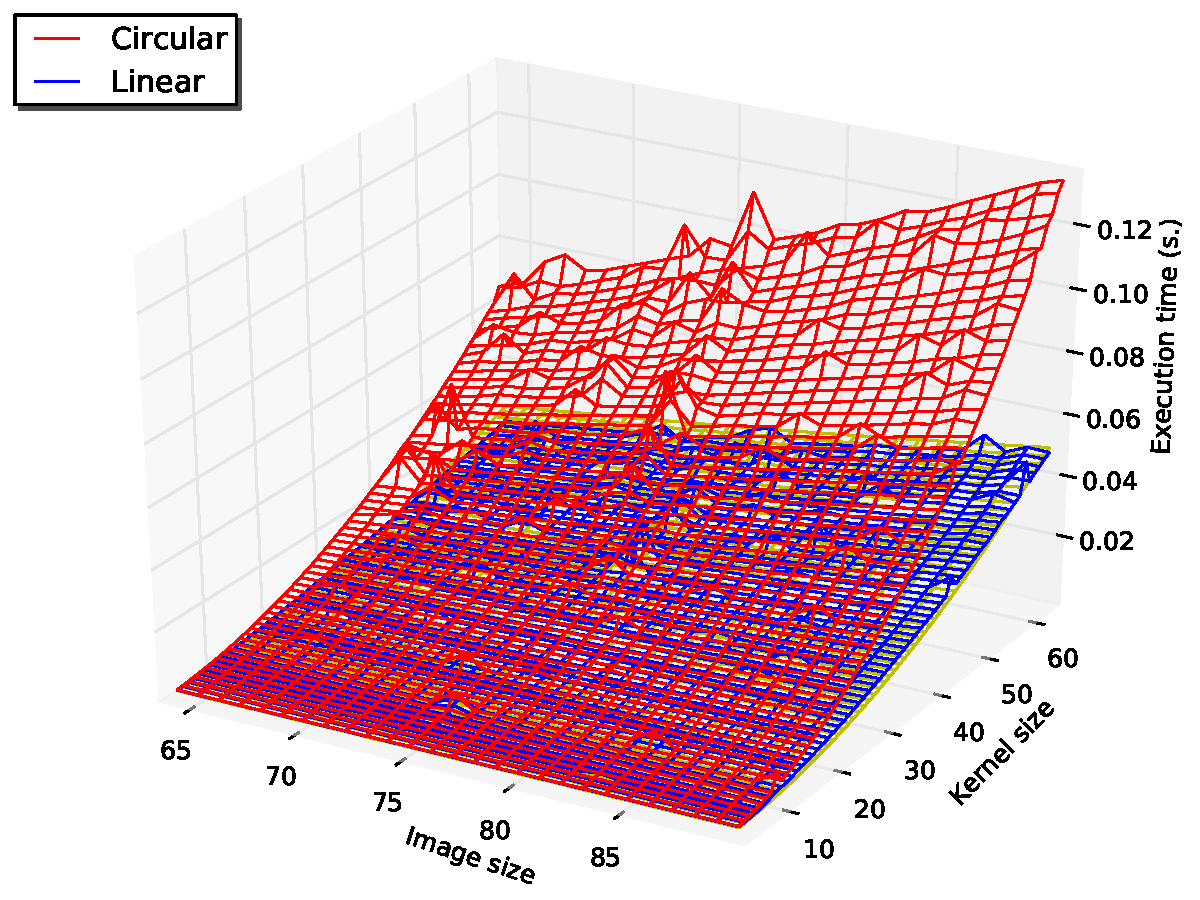
\includegraphics[width=0.5\linewidth]{../Images/benchmark_std_convolution.pdf}
\caption{\label{fig:benchmark_std_convolution.pdf} Execution time for computing a linear or circular convolution in C++, using nested for loops, of two signals of size $N$ and $M$. The execution time for a circular convolution grows with $N \times M$. For the linear convolution, the sum is restricted on less indices, which leads to an execution time faster than $N \times M$}
\end{figure}

On the tested machine, these curves are well approximated by :
\begin{itemize}
\item $t = 5.8.10^{-9} N^{1.98} K^{1.93}$ for the circular convolution
\item $t = 1.5.10^{-9} N^{2.38} K^{1.56}$ for the linear convolution
\end{itemize}

In the following sections, we introduce the Discrete Fourier Transform and \emph{show} that it leads to an algorithm for computing a convolution product requiring only an order of $N \log N$ operations.\\

\subsection{Discrete Fourier Transform}

\subsubsection{Introduction}

The \href{http://en.wikipedia.org/wiki/Discrete_Fourier_transform}{Discrete Fourier Transform} of a discrete signal $f[n]$ of length $N$ is defined as : 
\begin{eqnarray}
\nonumber FT[f][k] = \hat{f}[k] = \sum_{n=0}^{N-1} f[n] e^{-\frac{2 i \pi k n}{N}}
\end{eqnarray}

The discrete fourier transform of a discrete signal of length $N$ is periodic of period $N$ :\\
\begin{eqnarray}
\nonumber \forall p \in \mathbb{Z}, \hat{f}[k+pN] &=& \sum_{n=0}^{N-1} f[n] e^{-\frac{2 i \pi (k+pN) n}{N}} \\
\nonumber                                        &=& \sum_{n=0}^{N-1} f[n] e^{-\frac{2 i \pi k n}{N} }e^{-\frac{2 i \pi p N n}{N}}\\
\nonumber                                        &=& \sum_{n=0}^{N-1} f[n] e^{-\frac{2 i \pi k n}{N}}e^{-2 i \pi p n}\\
\nonumber                                        &=& \hat{f}(k)
\end{eqnarray}
The inverse discrete fourier transform of a discrete frequency signal $\hat{f}[k]$ is defined as :
\begin{eqnarray}
\nonumber IFT[\hat{f}][n] = f[n] = \frac{1}{N} \sum_{k=0}^{N-1} \hat{f}[k] e^{\frac{2i\pi k n}{N}}
\end{eqnarray}
The scaling factor $\frac{1}{N}$ is required to get the true inverse. To check this, let's compute $IFT[FT[f]][n]$ to check it equals to $f[n]$ :
\begin{eqnarray}
\nonumber IFT[FT[f]][n] &=& \frac{1}{N} \sum_{k=0}^{N-1} FT[f][k]  e^{\frac{2i\pi k n}{N}} \\
\nonumber               &=& \frac{1}{N} \sum_{k=0}^{N-1} \sum_{m=0}^{N-1} \left( f[m] e^{-\frac{2 i \pi k m}{N}} \right)  e^{\frac{2i\pi k n}{N}}\\
\nonumber               &=& \frac{1}{N} \sum_{k=0}^{N-1} \sum_{m=0}^{N-1} f[m] e^{\frac{2i\pi k (n-m)}{N}} \\
\nonumber               &=& \frac{1}{N} \sum_{m=0}^{N-1} f[m] \sum_{k=0}^{N-1} e^{\frac{2i\pi k (n-m)}{N}}
\end{eqnarray}

The last sum equals $N$ when $n \equiv m[N]$ and $0$ otherwise since it is a geometric serie of common ratio $e^{\frac{2i\pi (n-m)}{N}}$ : \\
If $n \equiv m [N]$ (m is in [0, N-1]): $\sum_{k=0}^{N-1} (e^{\frac{2i\pi (n-m)}{N}})^k = \sum_{k=0}^{N-1} 1 = N$,\\
Otherwise : $\sum_{k=0}^{N-1} (e^{\frac{2i\pi (n-m)}{N}})^k = \frac{1 - (e^{\frac{2i\pi (n-m)}{N}})^N}{1 - e^{\frac{2i\pi (n-m)}{N}}} =  \frac{1 - e^{2i\pi (n-m)} }{1 - e^{\frac{2i\pi (n-m)}{N}}} = 0$.\\
From the previous result, we get : \\
\begin{eqnarray}
\nonumber IFT[FT[f]][n] &=& \frac{1}{N} \sum_{m=0}^{N-1} f[m] \sum_{k=0}^{N-1} e^{\frac{2i\pi k (n-m)}{N}}\\
\nonumber              &=& \frac{1}{N} (N . f[n \bmod N]) = f[n \bmod N]
\end{eqnarray}
Therefore : $IFT\mbox{ }o\mbox{ }FT = identity$ when restricted on the horizon [0,N-1]. In fact, we have built a periodic signal of period $N$ which is repetitions of $f$.\\

In terms of complexity, we need an order of $N^2$ operations to compute the DFT of a signal of length $N$ ($N$ products for each of the $N$ components). In the following sections, we first show how we can compute a n-dimensional DFT from only 1D DFT and then briefly introduces the Fast Fourier Transform which decreases the number of required operations down to an order of $N \log N$ for a performing a DFT of a signal of length $N$.

\subsubsection{Computing a 2D Fourier transform from 1D Fourier transforms}

A 2D Fourier transform can be computed from 1D fourier transforms. For sake of simplicity, let's write $w_P = e^{\frac{-2i\pi}{P}}$. The 2D Fourier Transform of a signal $s[n,m]$ of size $(N,M)$ is defined as :
\begin{eqnarray}
S[k,j] &=& \sum_{n=0}^{N-1} \sum_{m=0}^{M-1} s[n,m] e^{\frac{-2i\pi jm}{M}}e^{\frac{-2i\pi kn}{N}}\\
       &=& \sum_{n=0}^{N-1} \sum_{m=0}^{M-1} s[n,m] w_M^{jm} w_N^{kn}\\
       &=& \sum_{n=0}^{N-1} (\sum_{m=0}^{M-1} s[n,m] w_M^{jm}) w_N^{kn}
\end{eqnarray}
It turns out that the 2D DFT can be computed by performing a 1D DFT on the rows of $s$ (the inner sum is on $n$ fixed) followed by a 1D DFT on the columns of the result. Let's denote $\hat{S}[n,j]$ the 2D signal for which the row $n$ holds the 1D DFT of the line $n$ of the original signal $s[n,m]$ :
\begin{equation}
\hat{S}[n,j] = \sum_{m=0}^{M-1} s[n,m] w_M^{jm}
\end{equation}
We can write :
\begin{equation}
S[k,j] = \sum_{n=0}^{N-1} \hat{S}[n,j] w_N^{kn}
\end{equation}
The previous equation corresponds to a 1D DFT performed on the columns of $\hat{S}$. Therefore, to compute a 2D DFT of $s$ you need to :
\begin{enumerate}
\item Perform a 1D DFT on the rows of $s$ which leads to the 2D signal $\hat{S}$
\item Perform a 1D DFT on the columns of $\hat{S}$
\end{enumerate}
The two previous operations can be done in the reverse order, no matter. This way of computing a 2D DFT from 1D DFTs is interesting because you can now compute DFT of n-dimensional signals involving only 1D-DFTs.

\subsubsection{Computing 2 DFT at once}

When we will apply the DFT to compute convolution products, we will need to compute two DFT : one for the image and one for the kernel. In fact, two DFTs can be simply computed with only one DFT. Given $f$ and $g$ are real signals, you can combine them to form a complex signal $h[n] = f[n] + i g[n]$. Given the DFT is linear : $FT[h][k] = FT[f][k] + i FT[g][k]$. The individual DFTs $FT[f]$ and $FT[g]$ are not the real and imaginary parts of $FT[h]$ given that the components of the DFTs are complex numbers. However, you know that :
\begin{eqnarray}
\nonumber f[n] = \frac{h[n] + (h[n])^*}{2} \\
\nonumber g[n] = \frac{h[n] - (h[n])^*}{2i} 
\end{eqnarray}
where $c^*$ is the conjugate of the complex number $c$. Therefore, you can write :
\begin{eqnarray}
\nonumber FT[f][k] = \frac{FT[h][k] + FT[h^*][k]}{2} \\
\nonumber FT[g][k] = \frac{FT[h][k] - FT[h^*][k]}{2i} 
\end{eqnarray}
It is possible to express $FT[h^*][k]$ in terms of $FT[h][k]$ by simply observing that :
\begin{eqnarray}
\nonumber FT[h^*][k] &=& \sum_{n=0}^{N-1} h^*[n] w_N^{k n} = \sum_{n=0}^{N-1} h^*[n] w_N^{k n}w_N^{-N n}\\
\nonumber            &=& \sum_{n=0}^{N-1} h^*[n] w_N^{-(N-k) n} = (\sum_{n=0}^{N-1} h[n] w_N^{(N-k) n})^*\\
\nonumber            &=& (FT[h][N-k])^*
\end{eqnarray}

We finally get :
\begin{eqnarray}
\nonumber \forall k \in [1, N-1] FT[f][k] = \frac{FT[h][k] + (FT[h][N-k])^*}{2} , FT[f][0] = \mbox{Re}(FT[h][0])\\
\nonumber \forall k \in [1, N-1] FT[g][k] = -i\frac{FT[h][k] - (FT[h][N-k])^*}{2}, FT[g][0] = \mbox{Im}(FT[h][0])
\end{eqnarray}

This technique is not required if you want to convolve several images with the same kernel since, in that case, you can precompute the DFT of the kernel one for all.

\subsubsection{Fast Fourier Transform}

To compute a DFT according to the previous definition, we need an order of $N^2$ operations. There are some efficient algorithms that have been designed, which involve only an order of $N \log N$ operations. They are called Fast Fourier Transform algorithms. We do not provide here how they work but just some pointers to some of the FFT algorithms~:
\begin{itemize}
\item Cooley-Tukey algorithm (\href{http://en.wikipedia.org/wiki/Cooley%E2%80%93Tukey_FFT_algorithm}{Wikipedia}) : breaks down a DFT of size $N = N_1 N_2$ into two DFT of size $N_1$ and $N_2$
\item Prime-factor algorithm (\href{http://en.wikipedia.org/wiki/Prime-factor_FFT_algorithm}{Wikipedia}) : breaks down a DFT of size $N = N_1 N_2$ into two DFT of size $N_1$ and $N_2$ when $N_1$ and $N_2$ have no common factors
\item Rader's algorithm (\href{http://en.wikipedia.org/wiki/Rader%27s_FFT_algorithm}{Wikipedia})
\item Winograd's algorithm
\end{itemize}
For the divide-and-conquer like algorithms (Cooley-Tukey, Prime-Factor), computing a DFT of a signal of size $N$ can be done by computing fourier transforms of smaller sizes, in particular of sizes which correspond to the prime factors of $N$. Quite a lot of details can be found in the documentation of the GSL on FFT algorithms (take the archive online and browse in the doc directory to find the file fft\_algorithms.texi) (see also the \href{http://www.gnu.org/software/gsl/manual/html_node/FFT-References-and-Further-Reading.html}{GSL documentation} for some pointers). The FFTW library makes use of the Cooley-Tukey algorithm, the prime factor algorithm, Rader's algorithm for prime sizes, and a split-radix algorithm and they also propose a generator of adhoc FFT algorithms for specific sizes, which, according to their documentation "produces new algorithms that we do not completely understand".

\subsubsection{Computational complexity}

There are several librairies providing optimized methods for computing a DFT. To cite only two of them : the \href{http://www.gnu.org/software/gsl}{GSL (Gnu Scientific Library)} and \href{http://www.fftw.org}{\nolinkurl{FFTW3}}. Others are cited on the \href{http://www.fftw.org/benchfft/ffts.html}{FFTW website}. The GSL proposes only 1D fourier transforms while FFTW3 proposes ND Fourier transforms. Therefore, for GSL, we will use the method presented in the previous section to compute a 2D Fourier Transform using only 1D Fourier transform. The scripts used to compute the Fourier Transform with the GSL and FFTW3 are \verb?fft_gsl.cc? and \verb?fft_fftw.cc?.\\

\begin{figure}[htbp]
\center 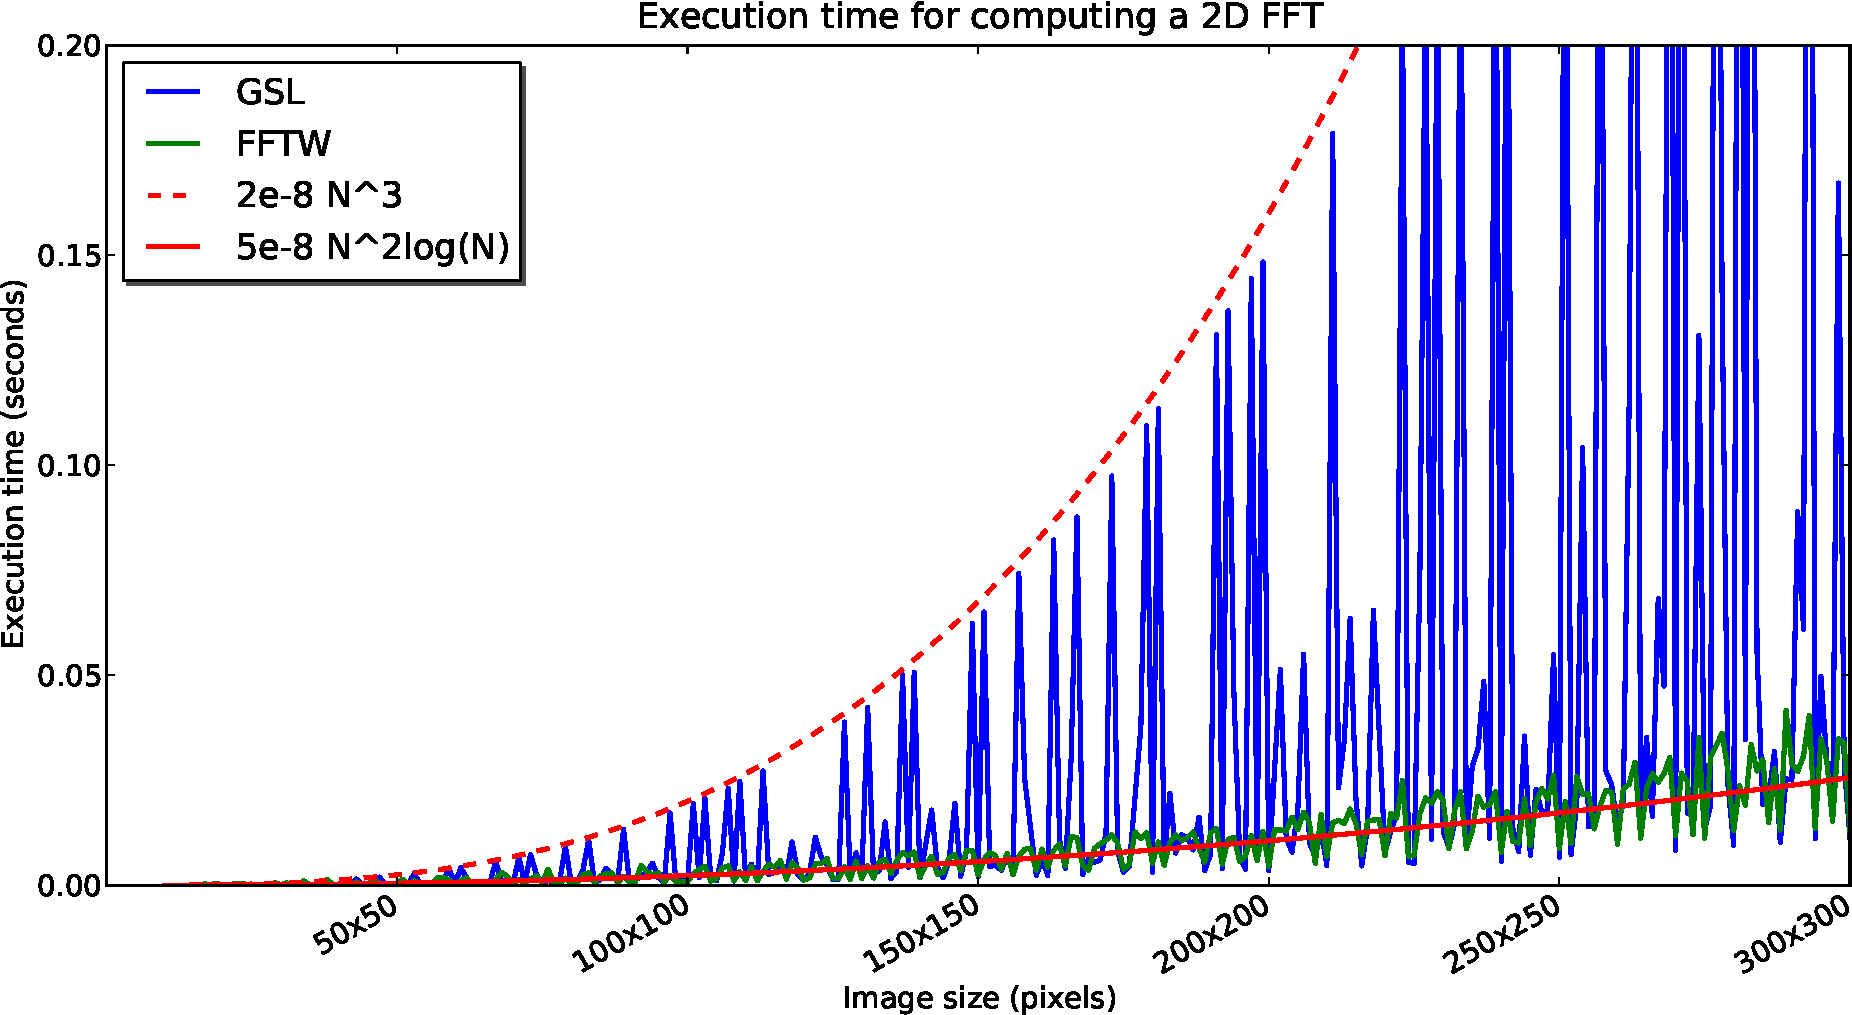
\includegraphics[width=0.6\linewidth]{../Images/test_fft-crop.pdf}
\caption{\label{fig:test_fft.pdf} Execution time for computing a 2D FFT. With a signal of size $NxN$, the performancs of the FFTW is well approximated with a curve in $N^2 \log(N)$ while the performances of the GSL sometimes reach $(N^2)^{3/2}$.}
\end{figure}

The image \ref{fig:test_fft.pdf} shows the time it takes, on an AMD Opteron 175, to compute the 2D-FFT for different signal sizes, the signals being randomly generated. The execution time fits with a $N \log(N)$ relationship. For some sizes, the GSL is performing worse than this relationship. The possible reason for this comes from how the GSL and the FFTW compute the FFT. As explained before, the algorithms rely on a factorization of the size of the signal. With the GSL, the implemented factors are $2,3,4,5,6,7$ (see \href{http://www.gnu.org/software/gsl/manual/html_node/Mixed_002dradix-FFT-routines-for-complex-data.html}{GSL website}) and for FFTW the implemented factors are $2,3,5,7,11,13$ (see \href{http://www.fftw.org/fftw3_doc/Complex-DFTs.html#Complex-DFTs}{FFTW website}). For the GSL, and apparently not the FFTW, if the size of the signal is not a product of only these factors, the performances can be worse than $N \log(N)$. In particular, this is the case for large prime numbers. If we look at the sizes where the performances are bad, they correspond to sizes like : 127x127, 131x131, .., 157x157, .. which are all prime numbers. It seems that FFTW handles successfully these large prime numbers.\\

\pagebreak

\section{2D Convolution product using the Discrete Fourier Transform}
\subsection{Introduction}

In the previous sections, we introduced the linear and circular convolutions as well as the Fourier transform with its efficient implementation of the Fast Fourier Transform. Here, we detail the link between the fourier transform and the convolution product. 

\subsubsection{Convolution theorem : circular convolution and fourier transform}

Consider we want to convolve an image of size $(N,N)$ with a filter of the same size $(N,N)$. As we saw in the introduction, a direct implementation of the convolution product with nested for loops requires an order of $N^2 N^2$ operations. It is possible to speed up this computation by using the Fourier transform. This relies on the \href{http://en.wikipedia.org/wiki/Convolution_theorem}{the convolution theorem} : the circular convolution product of two signals equals the inverse Fourier transform of the product of the fourier transforms of the signals :
\begin{myTheorem}
Let $f$ and $g$ be two discrete sequences of length $N$. The inverse fourier transform of the product of the fourier transform of $f$ and $g$ equals the circular convolution of $f$ and $g$ :
\begin{equation*}
\forall n \in [0,N-1], (f \circledast_N g)[n] = IFT[ FT[f] . FT[g] ][n]
\end{equation*}
\end{myTheorem}

To show this, let's compute the fourier transform of the circular convolution of $f[n]$ and $g[n]$ :
\begin{eqnarray}
FT[ f \circledast_N g ][k] &=& \sum_{i=0}^{N-1} \left( (f \circledast_N g)[i] w_N^{ki} \right)\\
			   &=& \sum_{i=0}^{N-1} \left(\sum_{j=0}^{N-1} f[(i-j) \bmod N].g[j] w_N^{ki}\right)\\
                           &=& \sum_{j=0}^{N-1} \left(g[j] \sum_{i=0}^{N-1} f[(i-j) \bmod N]. w_N^{ki}\right)\\
			   &=& \sum_{j=0}^{N-1} \left(g[j] w_N^{kj} \sum_{i=0}^{N-1} f[(i-j) \bmod N]. w_N^{k(i-j)}\right)\\
\end{eqnarray}
The index of the inner sum can be changed to get rid of $j$ since : 
\begin{equation}
\forall j \in [0,N-1], \{ (i-j) \bmod N, i=0..(N-1)\} = \{ i, i=0..(N-1)\}
\end{equation}
Therefore :
\begin{eqnarray}
FT[ f \circledast_N g ][k] &=& \sum_{j=0}^{N-1} \left(g[j] w_N^{kj} \sum_{i=0}^{N-1} f[i]. w_N^{ki} \right)\\
                           &=& \left( \sum_{i=0}^{N-1} f[i].w_N^{ki}\right) \left(\sum_{j=0}^{N-1} g[j] w_N^{kj}\right)\\
                           &=& FT[f][k] . FT[g][k]
\end{eqnarray}
Using the inverse fourier transform, we finally get the convolution theorem. Computing a convolution product that way requires to compute 2 DFTs, their product, and an inverse DFT. As we saw previously, when one needs to compute 2 DFT of real signals, they can be computed using a single DFT. Also, computing the DFT of a signal of $N$ requires an order of $N \log(N)$ operations. Adding the element-wise products, we get an algorithm for computing a convolution in $N (1+\log(N))$. This is a significant improvement compared to the naive implementation which requires an order of $N^2$ operations.

\subsubsection{Circular convolution of signals of different sizes}

In the previous section, we saw that the circular convolution of two signals of same size can be efficiently computed with the Fourier Transform. What to do with the circular convolution of two signals of different size ?\\

Let's consider the circular convolution of two signals $f$ and $g$ of respectively size $N$ and $M$ if $N \neq M$. Let's first consider the case $N > M$ which is usually the case when one wants to filter an image for example. Denote $g_\infty$ the signal $g$ padded with zeros on both sides :
\begin{equation}
\forall n, g_\infty[n] = \left\lbrace
\begin{array}{ccc}
g[n]     & \mbox{if} & 0 \leq n \leq M-1\\
0  & \mbox{otherwise}\\
\end{array}\right. \\
\end{equation}
Let's compute the Fourier Transform of $f$, $g_N$ and their pointwise product, as we did before but in the reverse order~:
\begin{eqnarray}
\forall k \in [0,N-1], FT[f][k].FT[g_\infty][k] &=& \left(\sum_{i=0}^{N-1} f[i] w_N^{ki}\right) \left( \sum_{j=0}^{N-1} g_\infty[j] w_N^{kj}\right)\\
                                           &=& \sum_{i=0}^{N-1} \left( \sum_{j=0}^{N-1} f[(i-j) \bmod N] g_\infty[j] w_N^{ki} \right)\\
				           &=& \sum_{i=0}^{N-1} \left( \sum_{j=0}^{M-1} f[(i-j) \bmod N] g[j] w_N^{ki} \right)\\
					   &=& \sum_{i=0}^{N-1} (f \circledast_N g)[i] w_N^{ki} \\
					   &=& FT[f \circledast_N g][k]
\end{eqnarray}

Let's now consider the second case, when $M > N$. Let's rewrite sligthly the circular convolution in this case in order to get a circular convolution of two signals of the same size $N$ :
\begin{eqnarray}
\forall k \in [0,N-1] (f \circledast_N g)[k] &=& \sum_{i=0}^{M-1} f[(k-i) \bmod N] g[i]\\
                                             &=& \sum_{i=0}^{N-1} f[(k-i) \bmod N] \sum_{p=0}^{\lceil \frac{M}{N}\rceil} g_\infty[i + pN]
\end{eqnarray}
The $\lceil x \rceil$ denotes the smallest integer larger than $x$. Let's denote $g_N$ the following signal, of size $N$ :
\begin{equation}
\forall n \in [0,N-1], g_N[n] = \sum_{p=0}^{\lceil \frac{M}{N}\rceil} g_\infty[i + pN]
\end{equation}
This signal is nothing more than slices of $g$, of size $N$ that we add together (see fig. \ref{fig:slice_g}). We can then write the circular convolution of $f$ and $g$ as a circular convolution of two signals of size $N$ which we can compute using the Fourier Transform.

\pagebreak
\subsubsection{Circular convolution : summary}

As a summary, we can now link the circular convolution as defined by equation \ref{eq:circular_convolution} with the Fourier Transform :
\begin{myTheorem}
Let $f$ and $g$ be two discrete sequences of respectively size $N$ and $M$. The circular convolution of $f$ and $g$, of size $N$, defined by $\forall k \in [0,N-1], (f\circledast g)[k] = \sum_{i=0}^{M-1} f[(k-i) \bmod N] g[i]$ can be computed using the Fourier Transform :
\begin{equation*}
\forall k \in [0,N-1], (f\circledast g)[k] = IFT[FT[f] . FT[\tilde{g}]][k]
\end{equation*}
with :
\begin{equation*}
\forall k \in [0,N-1] \tilde{g}[k] =
 \begin{cases}
 g_\infty[k] & \mbox{ if $M \leq N$} \\
 \sum_{p=0}^{\lceil \frac{M}{N}\rceil} g_\infty[k + pN]
 \end{cases}
\end{equation*}
and 
\begin{equation*}
\forall k, g_\infty[k] = \left\lbrace
\begin{array}{ccc}
g[k]     & \mbox{if} & 0 \leq k \leq M-1\\
0  & \mbox{otherwise}\\
\end{array}\right. \\
\end{equation*}
\end{myTheorem}

\subsubsection{Linear convolutions : particular cases of circular convolution}

We now want to adress the question of computing a linear convolution with the Fourier Transform. Answering this question is quite easy. If we look at the illustrations of the linear and circular convolutions (figures \ref{fig:linear_convolution} and \ref{fig:circular_convolution}), we see that the expression of the components of the two convolutions are the same if, in the case of a circular convolution instead of padding $f$ with wrapped around values we padd it with zeros. More formally, let's suppose we want to linearly convolve two signals $f$ and $g$ of respectively size $N$ and $M$. Let's now build the signal $f_M$, of size $N+M-1$ as:
\begin{equation*}
\forall k \in [0,N+M-2], f_M[k] = \left\lbrace
\begin{array}{ccc}
f[k]     & \mbox{if} & 0 \leq k \leq N-1\\
0  & \mbox{otherwise}\\
\end{array}\right. \\
\end{equation*}
The $f_M$ signal is somehow our $f_\infty$ but here defined as a finite sequence. The circular convolution of $f_M$ and $g$ gives :
\begin{eqnarray}
\forall k \in [0,N+M-2], (f_M \circledast_{N+M-1} g)[k] &=& \sum_{i=0}^{M-1} f_M[(k-i) \bmod (N+M-1)] g[i]
\end{eqnarray}
Given $i \in [0,M-1]$ and $k \in [0,N+M-2]$, then $k-i \in [-M+1, N+M-2]$. When $k-i$ is negative ($k-i \in [-M+1,-1]$), the wrap around leads to consider the indices $N \leq k-i+N+M-1 \leq N+M-2$ where $f_M$ is null. Also, for $k \in [N;N+M-2]$, there are some indices $k-i$ which fall on parts where $f_N$ is zero, in particular, when $k-i \in [N,N+M-2]$. Overall, the sum can be restricted to the indices $i$ where $k-i \in [0, N-1]$ and $i \in [0,M-1]$, which means $i \in [0,M-1] \cap [k-N+1,k]$ :
\begin{eqnarray}
\forall k \in [0,N+M-2], (f_M \circledast_{N+M-1} g)[k] &=& \sum_{i=\max(0, k-N+1)}^{\min(M-1,k)} f_M[(k-i) \bmod (N+M-1)] g[i]\\
							&=& \sum_{i=\max(0, k-N+1)}^{\min(M-1,k)} f[k-i] g[i]
\end{eqnarray}
Now, we just need to change the summation index :
\begin{eqnarray}
\nonumber \max(0,k-N+1) \leq i \leq \min(M-1,k) &\Longleftrightarrow& k - \min(M-1,k) \leq k-i \leq k - \max(0,k-N+1)\\
\nonumber                                       &\Longleftrightarrow& \max(k-M+1, 0) \leq k-i \leq \min(k, N-1)
\end{eqnarray}
Finally, we find the expression of the \textbf{Full} linear convolution (eq. \ref{eq:linear_convolution_full}):
\begin{equation*}
\forall k \in [0,N+M-2], (f_M \circledast_{N+M-1} g)[k] = \sum_{i=\max(0, k-M+1)}^{\min(N-1,k)} f[i] g[k-i] = h_f[k]
\end{equation*}


\pagebreak

If we want to compute the \textbf{Same} linear convolution (eq. \ref{eq:linear_convolution_same}), we need to pad the $f$ signal with slightly less zeros. In fact we need to pad the signal with at least $\frac{M}{2}$ zeros on one end;\\

\textbf{And restrict ???}\\



%As we saw in the previous section, using the DFT to perform a convolution leads to wrap around the image with $(N/2 + n -m)\mbox{ }mod\mbox{ }N$. To avoid the effect of this wrap-around, it is sufficient to pad the image with at least $\frac{N+1}{2}$ zeros. Let's suppose we want to compute the linear convolution of two discrete signals $f$ and $g$ of size $N$. Let's construct the signal $f_L$ which is the signal $f$ padded with $L \geq \frac{N+1}{2}$ zeros at the really end :
%\begin{eqnarray}
%\nonumber \forall n \in [0,N+L-1], f_L[n]=
%\left\lbrace
%\begin{array}{ccc}
%f[n]  & \mbox{if} & 0 \leq n \leq N-1\\
%0 & \mbox{otherwise}
%\end{array}\right.
%\end{eqnarray}
%And let's construct the signal $g_L$ which is the signal $g$, shifted in time, wrapped around and padded with $L$ zeros in the "middle" :
%\begin{figure}[htbp]
%\center 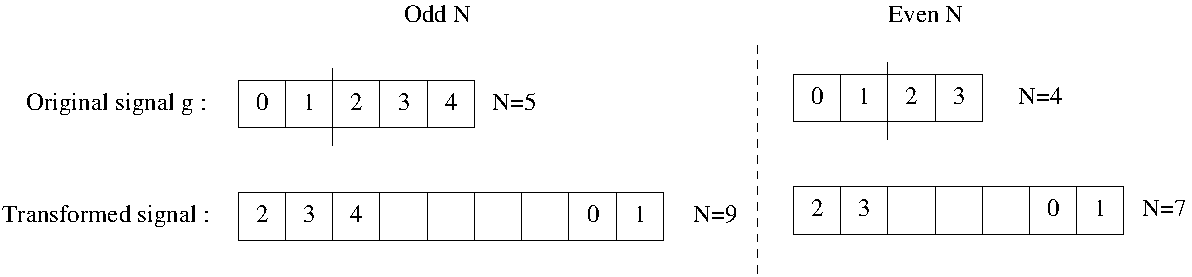
\includegraphics[width=\linewidth]{../Images/wrap_g.pdf}
%\end{figure}
%
%\begin{eqnarray}
%\nonumber \forall n \in [0,N+L-1], g_L[n]=
%\left\lbrace
%\begin{array}{ccc}
%g[N/2+n]  & \mbox{if} & 0 \leq n \leq \frac{N-1}{2}\\
%0 & \mbox{if} & \frac{N-1}{2}+1 \leq n \leq \frac{N-1}{2}+L\\
%g[n-(\frac{N+1}{2} + L)] & \mbox{if} & \frac{N-1}{2} + L + 1 \leq n \leq N+L-1
%\end{array}\right.
%\end{eqnarray}
%
%Therefore, we now have two signals $f_L$ and $g_L$ of size $N+L$. Let's now compute the inverse DFT of the product of the DFT of $f_L$ and $g_L$ :
%\begin{eqnarray}
%\nonumber \forall n \in [0, N+L-1], IFT[FT[f_L] . FT[g_L]][n] &=& \frac{1}{N+L} \sum_{m=0}^{N+L-1} \sum_{p=0}^{N+L-1} f_L[m] g_L[p] (\sum_{k=0}^{N+L-1} e^{\frac{2i\pi k (n - m -p)}{N+L}})\\
%\nonumber &=& \frac{1}{N+L} \sum_{m=0}^{N-1} \sum_{p=0}^{N+L-1} f_L[m] g_L[p] (\sum_{k=0}^{N+L-1} e^{\frac{2i\pi k (n - m -p)}{N+L}})\\
%\nonumber &=& \frac{1}{N+L} \sum_{m=0}^{N-1} \sum_{p=0}^{N+L-1} f[m] g_L[p] (\sum_{k=0}^{N+L-1} e^{\frac{2i\pi k (n - m -p)}{N+L}})\\
%\nonumber &=&\sum_{m=0}^{N-1} f[m] g_L[(n-m)\mbox{ }mod\mbox{ }(N+L)]\\
%\nonumber &=& A + B 
%\end{eqnarray}
%
%where, $A = \sum_{m=0}^{n} f[m] g_L[(n-m)\mbox{ }mod\mbox{ }(N+L)]$ and $B = \sum_{m=n+1}^{N-1} f[m] g_L[(n-m)\mbox{ }mod\mbox{ }(N+L)]$. Now, restrict the previous computation to $n \in [0,N-1]$. Therefore, for the first sum :
%\begin{eqnarray}
%\nonumber 0 \leq m \leq n, 0 \leq n \leq N-1 \Rightarrow 0 \leq n-m \leq N-1 < N + L
%\end{eqnarray}
%
%Therefore $(n-m)\mbox{ }mod\mbox{ }(N+L-1) = n-m$. Given $L \geq \frac{N+1}{2}$, we also have $\frac{N-1}{2}+L\geq N$ and $n-m \leq \frac{N-1}{2}+L$. Given the definition of $g_L$, we get three cases:
%\begin{small}
%\begin{eqnarray}
%\nonumber \forall m \in [0,n], g_L[(n-m)\mbox{ }mod\mbox{ }(N+L)]=
%\left\lbrace
%\begin{array}{ccc}
%g[N/2+n-m]  & \mbox{if} & 0 \leq n-m \leq \frac{N-1}{2} \\
%            & &\Rightarrow n - \frac{N-1}{2} \leq m \leq n\\
%0 & \mbox{if} & \frac{N-1}{2}+1 \leq n-m \leq \frac{N-1}{2}+L \\
%            & &\Rightarrow n - (\frac{N-1}{2}+L) \leq m \leq n - \frac{N-1}{2}-1\\
%g[n-m-(\frac{N+1}{2}+L)] &\mbox{if} & \frac{N-1}{2}+L+1 \leq n-m \leq N+L-1\\
%            & & \Rightarrow n - N - L + 1 \leq m \leq n - (\frac{N-1}{2} + L)-1
%\end{array}\right.
%\end{eqnarray}
%\end{small}
%Given that $L \geq \frac{N+1}{2}$, $n-(\frac{N-1}{2}+L)-1 \leq -1$. This last case is therefore never used given that $m \geq 0$. This allows to write :
%\begin{eqnarray}
%\nonumber A &=& \sum_{m=0}^{n} f[m] g_L[(n-m)\mbox{ }mod\mbox{ }(N+L)]\\
%\nonumber   &=& \sum_{m=\max(0,n - \frac{N-1}{2})}^{n} f[m] g[N/2+n-m]
%\end{eqnarray}
%Let's now consider the second sum :
%\begin{eqnarray}
%\nonumber n+1 \leq m \leq N-1, 0 \leq n \leq N-1 \Rightarrow  n - N + 1 \leq n-m \leq -1
%\end{eqnarray}
%
%and $n - N + 1 \geq  -N + 1 \geq -(L+N)+1$. This means that when $n+1 \leq m \leq N-1$, $n - m\mbox{ }mod\mbox{ }(N+L) = n-m+N+L$ and $n + L +1\leq n-m + N+L \leq N + L - 1$. Given that $L \geq \frac{N+1}{2}$, $n + L + 1\geq \frac{N+1}{2}$. This allows to write :
%\begin{footnotesize}
%\begin{eqnarray}
%\nonumber \forall m \in [n+1,N-1], g_L[(n-m)\mbox{ }mod\mbox{ }(N+L)]=
%\left\lbrace
%\begin{array}{ccc}
%\nonumber g[n-m + 3N/2 + L] &\mbox{if} & 0 \leq n-m+N+L \leq \frac{N-1}{2} \\
%\nonumber                      & & \Rightarrow n+L+\frac{N}{2}+1 \leq m \leq m+N+L\\
%\nonumber 0 & \mbox{if} &  \frac{N-1}{2}+1 \leq n-m+N+L \leq \frac{N-1}{2}+L\\
%\nonumber   &           &  \Rightarrow  n + \frac{N}{2}+1 \leq m \leq n + L + \frac{N}{2}\\
%\nonumber g[n - m +\frac{N}{2}]  & \mbox{if} & \frac{N-1}{2}+L+1 \leq n-m+N+L \leq N+L-1 \\
%\nonumber             & &\Rightarrow n + 1 \leq m \leq n+\frac{N}{2}
%\end{array}\right.
%\end{eqnarray}
%\end{footnotesize}
%Therefore, we can write :
%\begin{eqnarray}
%\nonumber B &=& \sum_{m=n+1}^{N-1} f[m] g_L[(n-m)\mbox{ }mod\mbox{ }(N+L)]\\
%\nonumber   &=& \sum_{m=n+1}^{\min(N-1,n+\frac{N}{2})} f[m] g[n-m+\frac{N}{2}]
%\end{eqnarray}
%Therefore, we finally get the result :
%\begin{eqnarray}
%\nonumber \forall n \in [0, N-1], IFT[FT[f_L] . FT[g_L]][n] &=& A + B\\
%\nonumber &=& \sum_{m=\max(0,n - \frac{N-1}{2})}^{n} f[m] g[\frac{N}{2}+n-m] \\
%\nonumber  &+& \sum_{m=n+1}^{\min(N-1,n+\frac{N}{2})} f[m] g[n-m+\frac{N}{2}]\\
%\nonumber &=& \sum_{m=\max(0,n - \frac{N-1}{2})}^{\min(N-1,n+\frac{N-1}{2})} f[m] g[n-m+\frac{N}{2}]\\
%\nonumber &=& (f * g)[n]
%\end{eqnarray}

\subsection{Speeding-up by padding}

Computing the DFT is faster for some specific sizes. There are some radix-2 algorithms working with images of sizes being a power of 2 but also mixed-radix algorithms which work with a factorization of the image's size. As we saw previously on figure \ref{fig:test_fft.pdf}, the performances can be really reduced if the image's size is non-optimal. In the two next paragaphs, we illustrate methods to change the size of the images to convolve in order to fall on optimal sizes for the FFT algorithms.\\

To determine if a size is optimal, we just factorize it and check if the factorization contains only factors for which sub-transforms are optimally computed. In GSL, this means only size that can be written $2^a*3^b*4^c*5^d*6^e*7^f$. In addition, it seems that when the size is a multiple of $4.4.4.2 = 128$, the mixed-radii algorithm does not perform a FFT efficiently. Therefore, all the sizes multiple of $128$ are considered non-optimal. In FFTW3, an optimal size is of the form $2^a*3^b*5^c*7^d*11^e*13^f$, with $e+f$ equals $0$ or $1$. We also discarder the sizes multiple of $4.4.4.2$ which also appeared to decrease the performances.\\

\subsubsection{Linear convolution}

To compute a linear convolution with the FFT, it is sufficient to pad the images with enough zeros, namely $\frac{N+1}{2}$. This bound is a lower bound. Therefore, we can pad the images with more than $\frac{N+1}{2}$ to get sizes that are optimally computed with the algorithm we use.\\

\begin{figure}[htbp]
\center 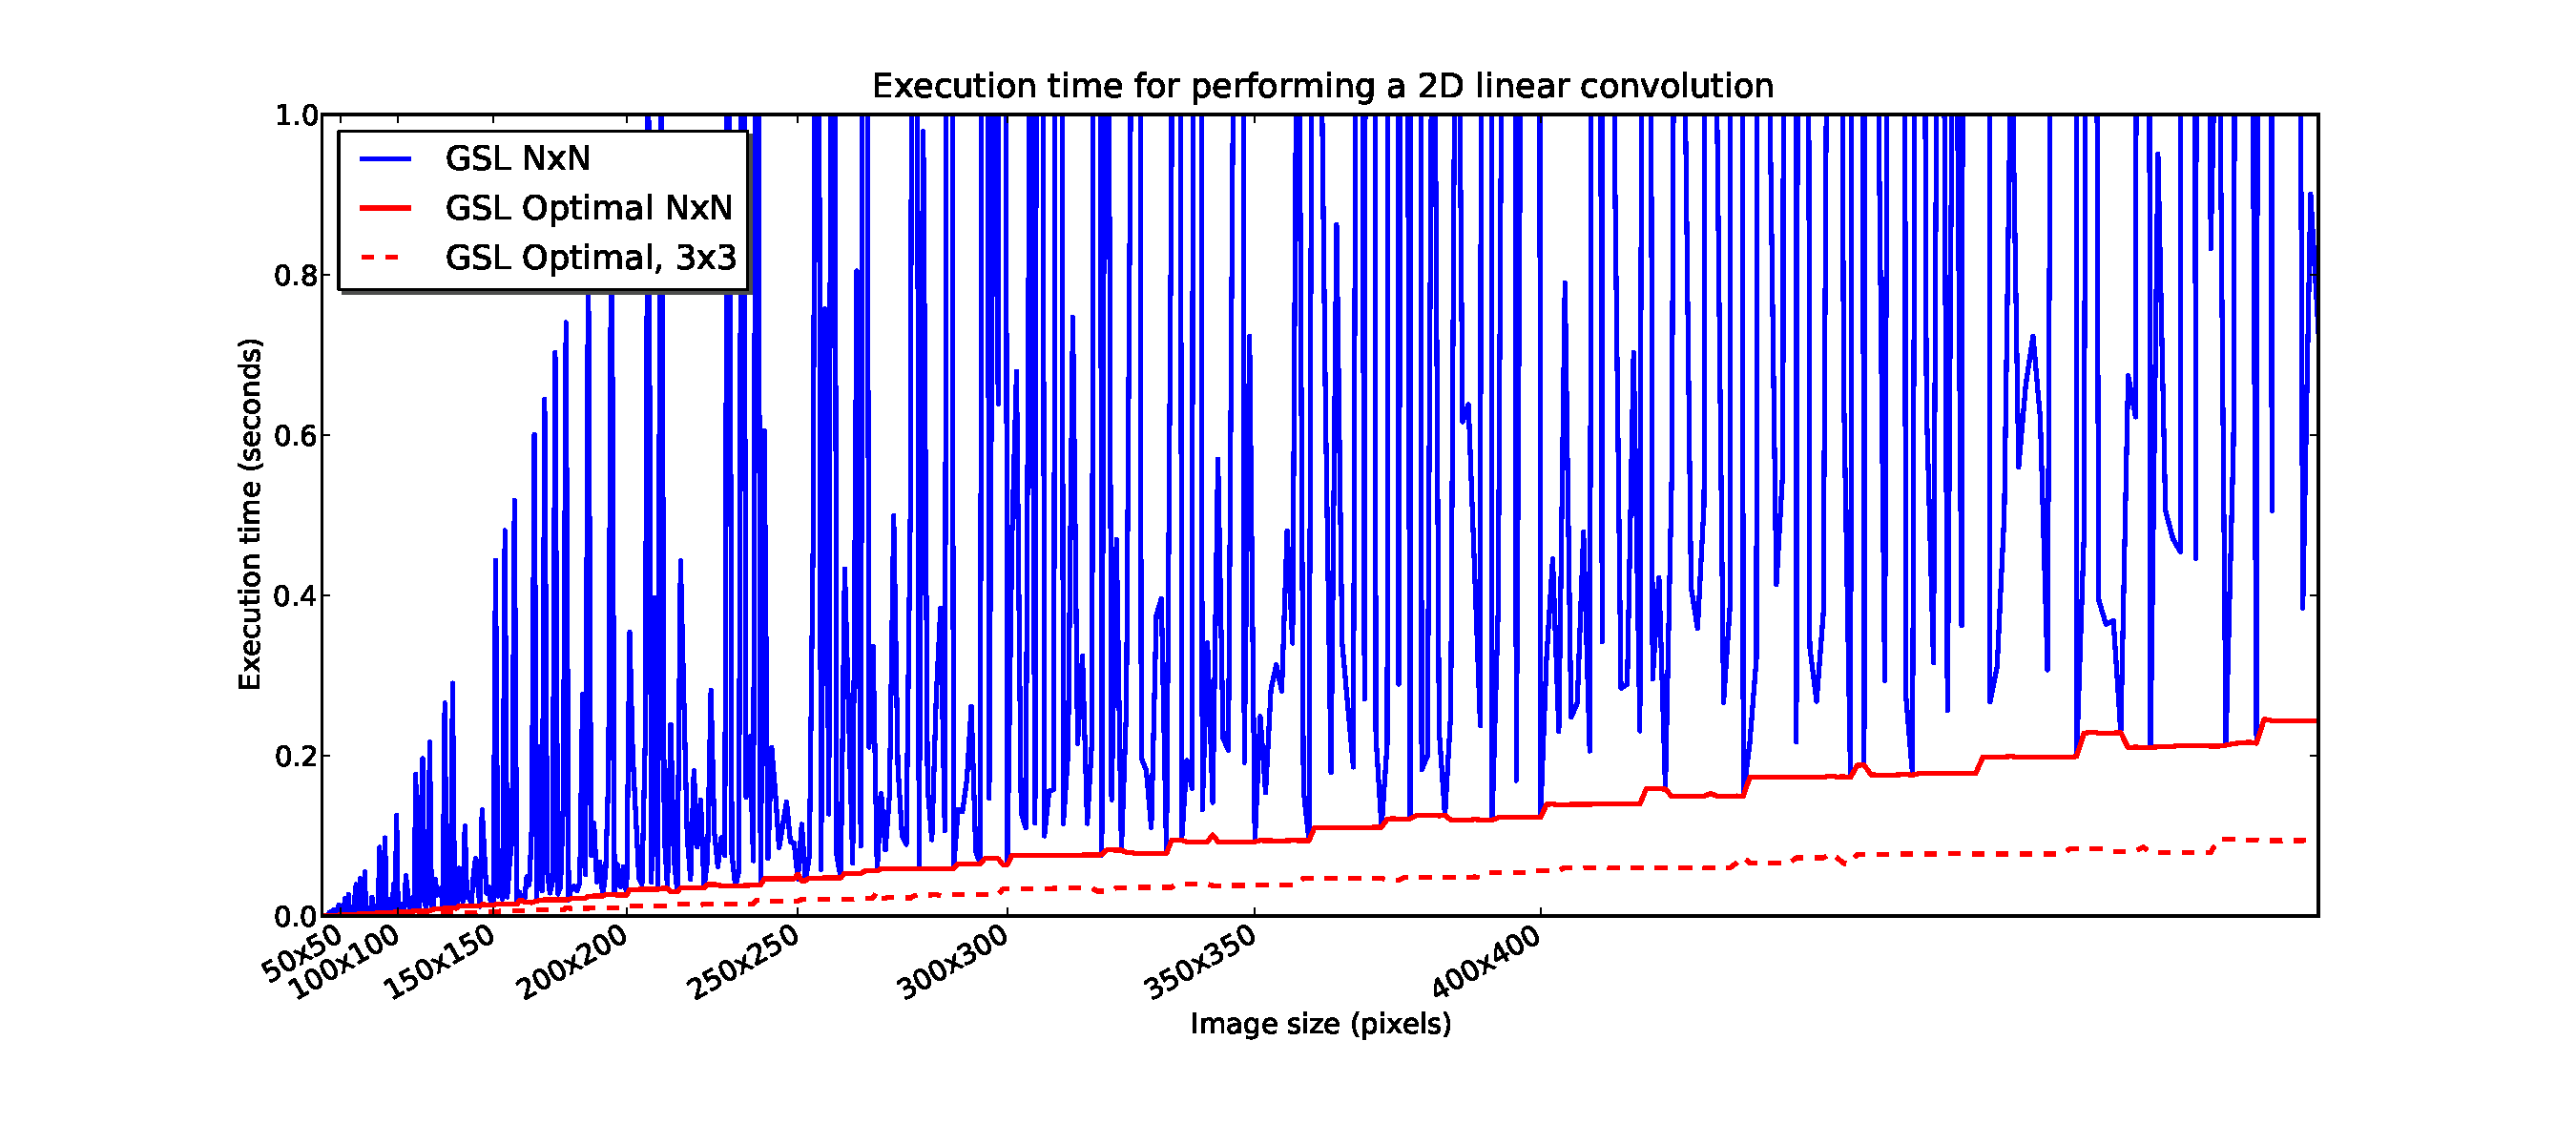
\includegraphics[width=0.75\linewidth]{../Images/benchmark_linear_convolution_gsl.pdf}
\caption{\label{fig:benchmark_linear_convolution_gsl.pdf}Execution time for performing a linear convolution with GSL. The times for both the unpadded and padded images are shown. Clearly, padding with zeros in order to get optimal sizes (in the sense of the factor decomposition of GSL) improves the performances.}
\end{figure}

The time it takes to compute a 2D linear convolution with or without padding, using the GSL (for which optimal sizes are of the form $2^a3^b4^c5^d6^e7^f$, see \href{http://www.gnu.org/software/gsl/manual/html_node/Mixed_002dradix-FFT-routines-for-complex-data.html}{GSL website}), is shown on the figure \ref{fig:benchmark_linear_convolution_gsl.pdf}. It computes a 2D linear convolution of 2 randomly generated images of the same size. Padding clearly improves the processing time of the convolution. For this illustration, we used a small x-axis increment to better appreciate the effect of non-optimal sizes. The dashed line represents the execution time when the kernel size is small (actually 3x3). Since padding depends on the size of the kernel, the kernel size influences the size of the FFTs to compute. For convenience, only the times of the optimal version with a small kernel are plotted. This illustration was generated with the results produced by this script : \href{http://jeremy.fix.free.fr/Software/Convolution/linear_convolution_gsl_benchmark.cc}{linear\_convolution\_gsl\_benchmark.cpp}\\

\begin{figure}[htbp]
\center 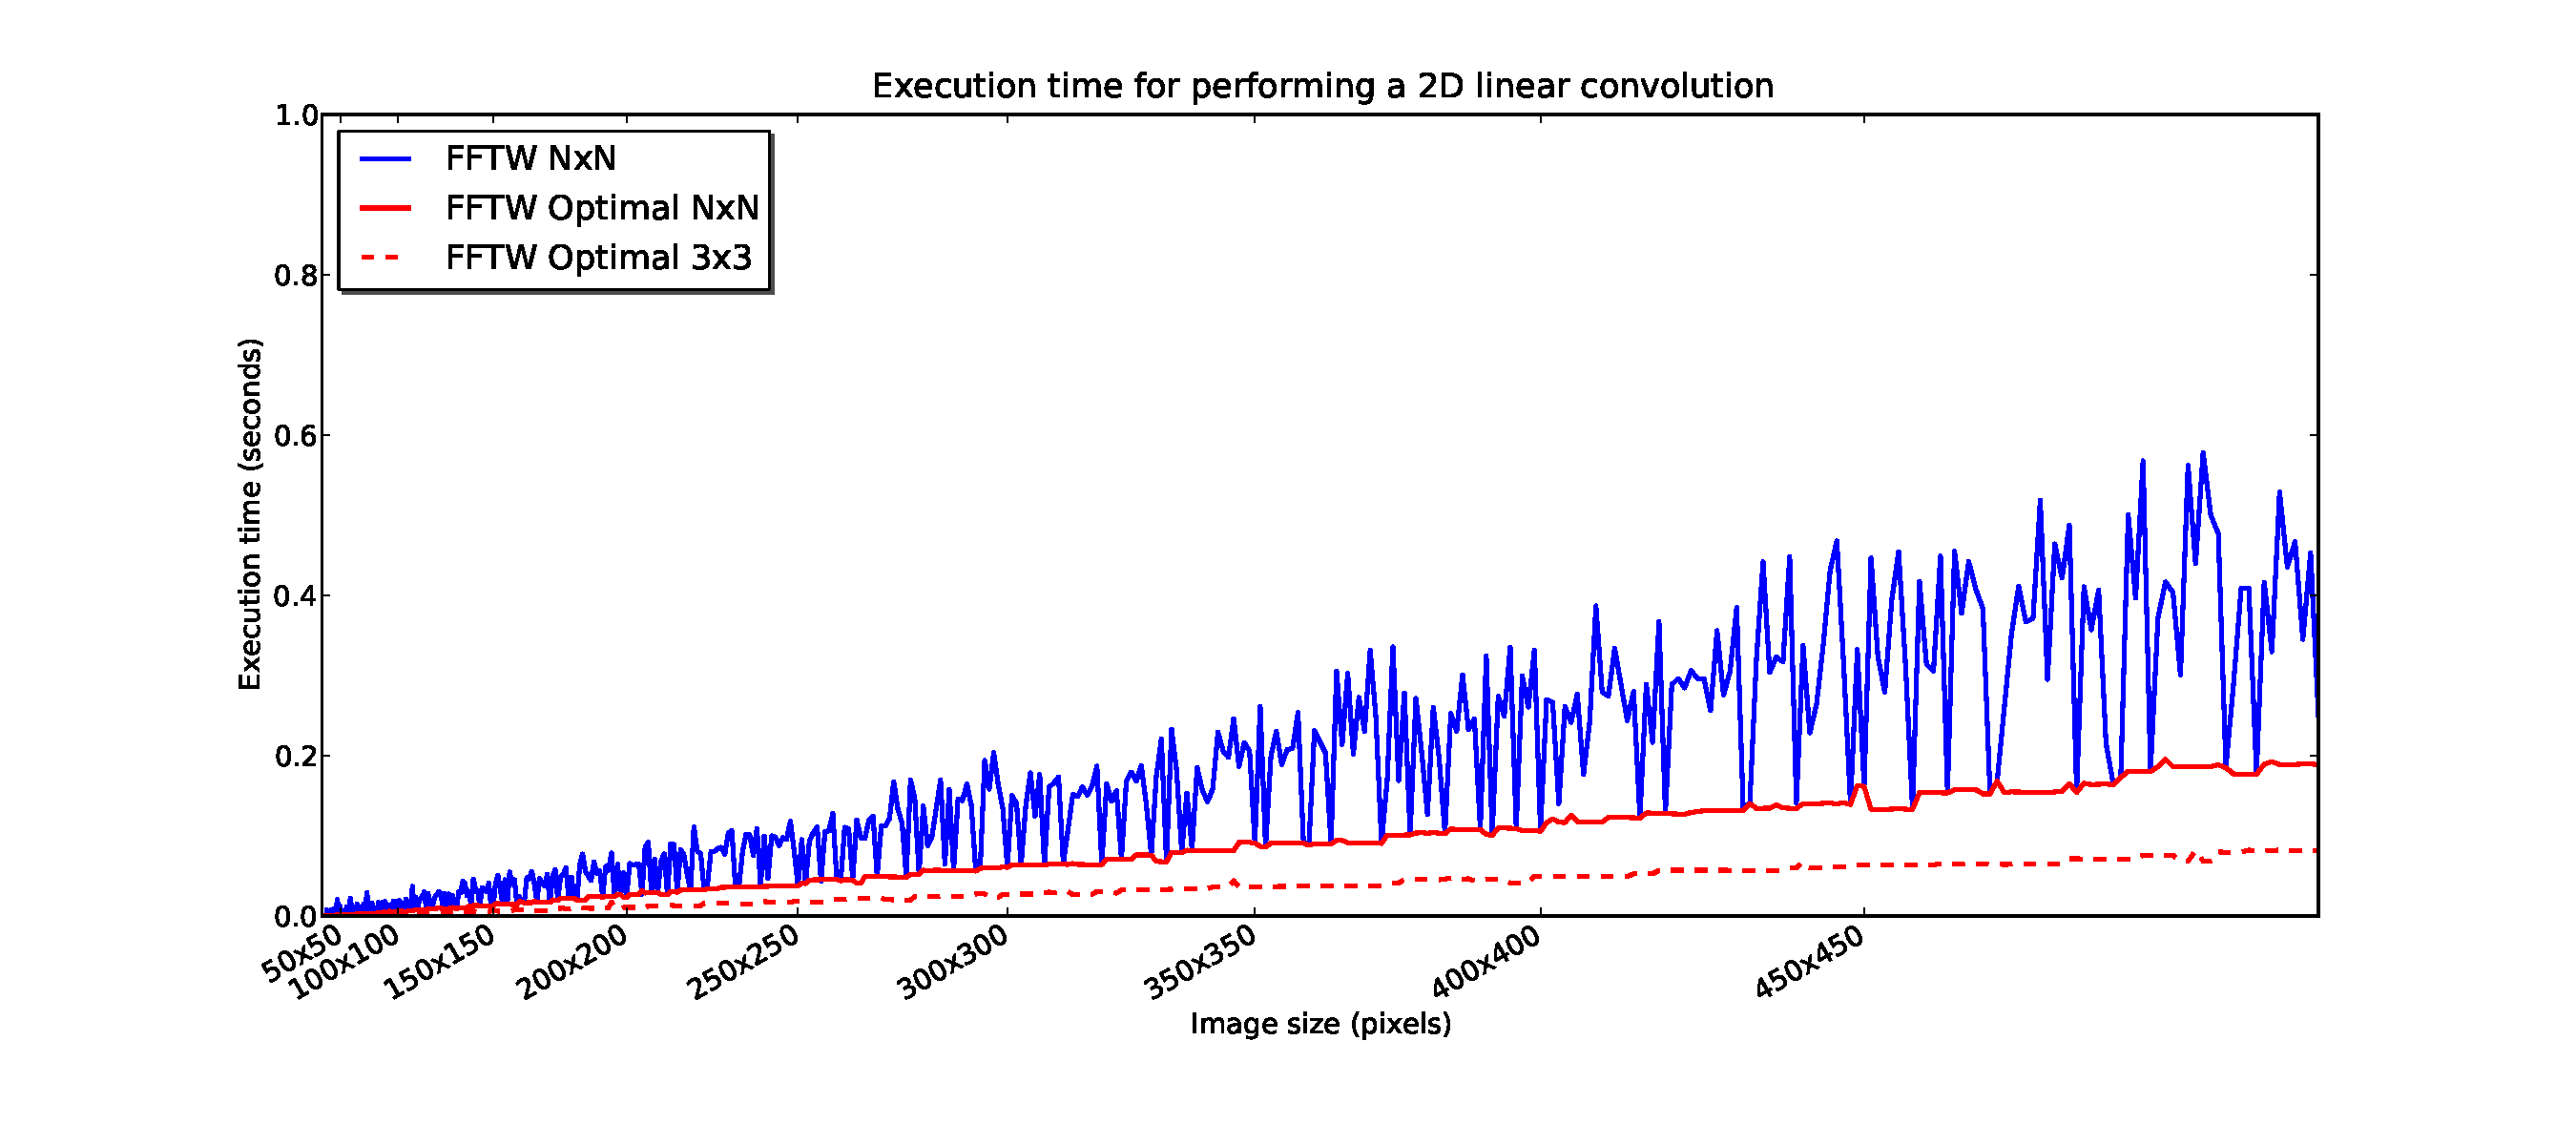
\includegraphics[width=0.85\linewidth]{../Images/benchmark_linear_convolution_fftw.pdf}
\caption{\label{fig:benchmark_linear_convolution_fftw.pdf}Execution time for performing a linear convolution with FFTW. The times for both the unpadded and padded images are shown. Clearly, padding with zeros in order to get optimal sizes (in the sense of the factor decomposition of FFTW) improves the performances.}
\end{figure}

The figure \ref{fig:benchmark_linear_convolution_fftw.pdf} shows the execution time for performing a 2D linear convolution with FFTW (for which optimal sizes are of the form $2,3,5,7,11,13$,see \href{http://www.fftw.org/fftw3_doc/Complex-DFTs.html#Complex-DFTs}{FFTW website}), with or without padding to get optimal sizes, using 2 randomly generated matrices of the same size. Again, we see that padding leads to better performances. This illustration was generated with the results produced by this script : \href{http://jeremy.fix.free.fr/Software/Convolution/linear_convolution_fftw_benchmark.cpp}{linear\_convolution\_fftw\_benchmark.cc}.\\

The figure \ref{fig:benchmark_linear_convolution_compare.pdf} compares the execution times with the GSL and FFTW implementations. The FFTW based implementation performs slightly better than the GSL implementation. It performs almost $20\%$ better as soon as the image size is at least $200 \times 200$. The performances of the GSL are not as bad as we may have thought when we observed the bad performances of the GSL computing a FFT. It is simply because we are interested in a convolution product, therefore we are not obliged to stick to some specific frequencies and we can pad the signal as we want in order to get optimally computed sizes.

\begin{figure}[htbp]
\center 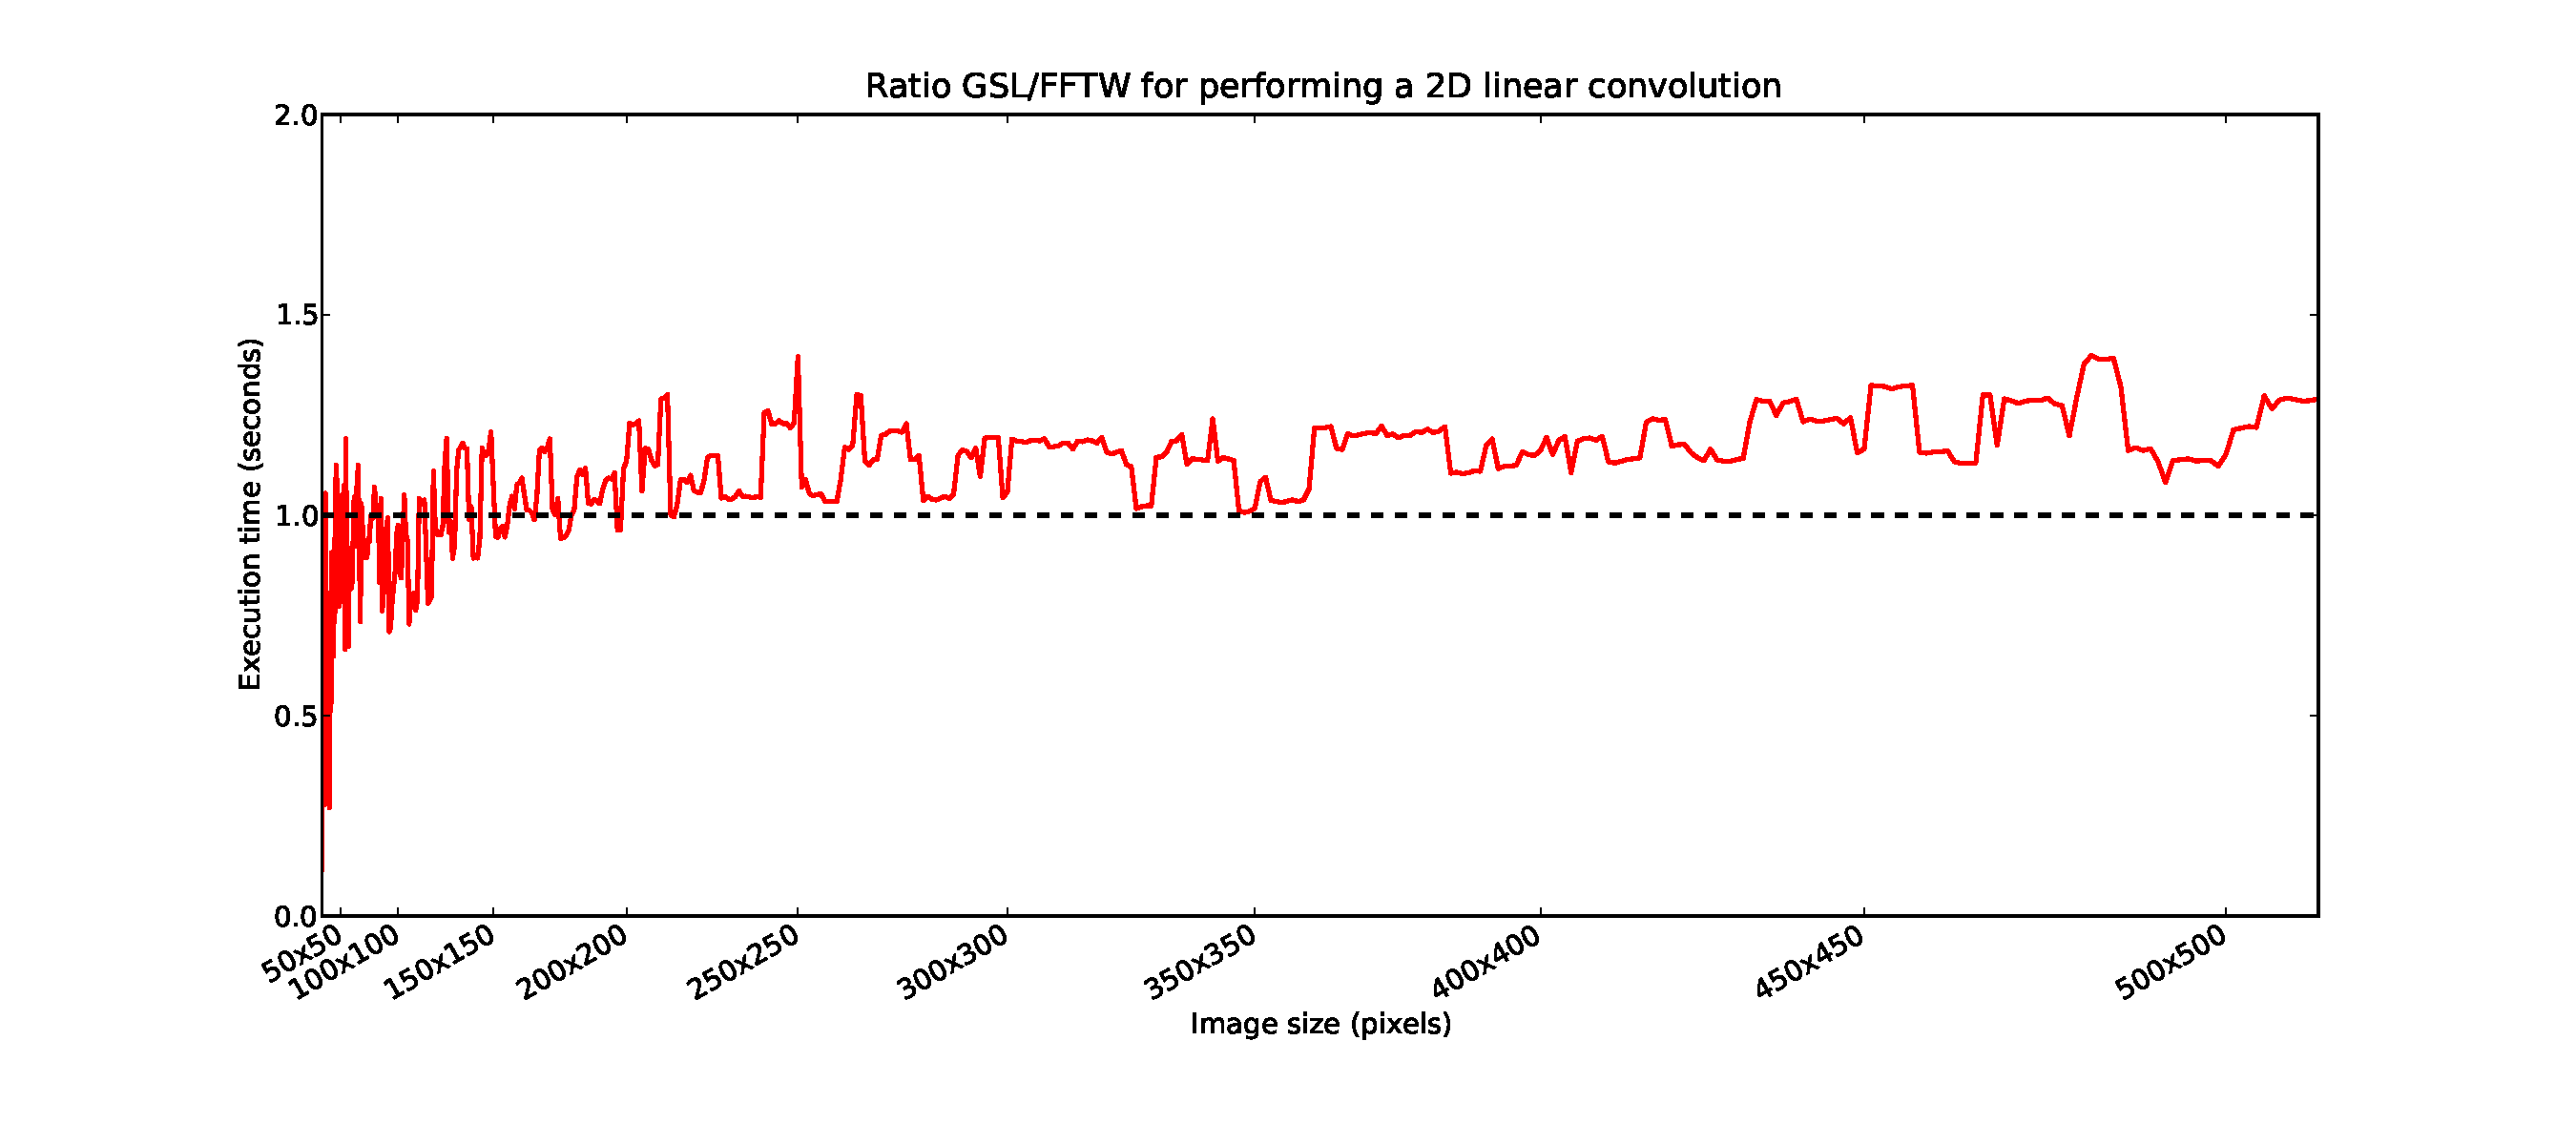
\includegraphics[width=0.85\linewidth]{../Images/benchmark_linear_convolution_compare.pdf}
\caption{\label{fig:benchmark_linear_convolution_compare.pdf}Comparison of the execution time for performing a linear convolution using optimal sizes with GSL or FFTW. The FFTW based implementation is slightly better, almost $20\%$ faster for sizes at least $200\times 200$.}
\end{figure}


\subsubsection{Circular convolution}

We can also change the size of an image to optimally compute a circular convolution. For a circular convolution, instead of padding with zeros on both sides, we pad the image with wrapped around values. We then use the FFT to compute a circular convolution and extract the central part of the resulting image. The excluded regions, on the border of the result, will be meaningless since they combine the wrapped around pixel values with themselves but they are anyway discarded. In the code, it is a bit longer to write because we need a complex array in which the source image and the kernel are copied respectively in the real and imaginary parts. As we will see, padding does not necessarily improves the performances. This is because a circular convolution can be computed without padding. As soon as we want to pad the images to perform a circular convolution, we must pad with at least the size of the kernel (half the size on both sides). This can seriously increase the size of the images for the FFT.\\

On figure \ref{fig:benchmark_circular_convolution_gsl.pdf} (again involving 2 randomly generated images of the same size), padding does not always lead to better performances. When the size of the image is optimal, it is clear that the padded version must be worse. However, when the size is not optimal, padding can or cannot improves the performances. In this case, it is not clear how to define a rule deciding when we should pad or when we should not. We may define a simple rule : if the size is optimal, do not pad, otherwise pad. We may also perform tests before-hand to check which version is faster but this is really dependent on the size of the images to convolve.\\

\begin{figure}[htbp]
\center 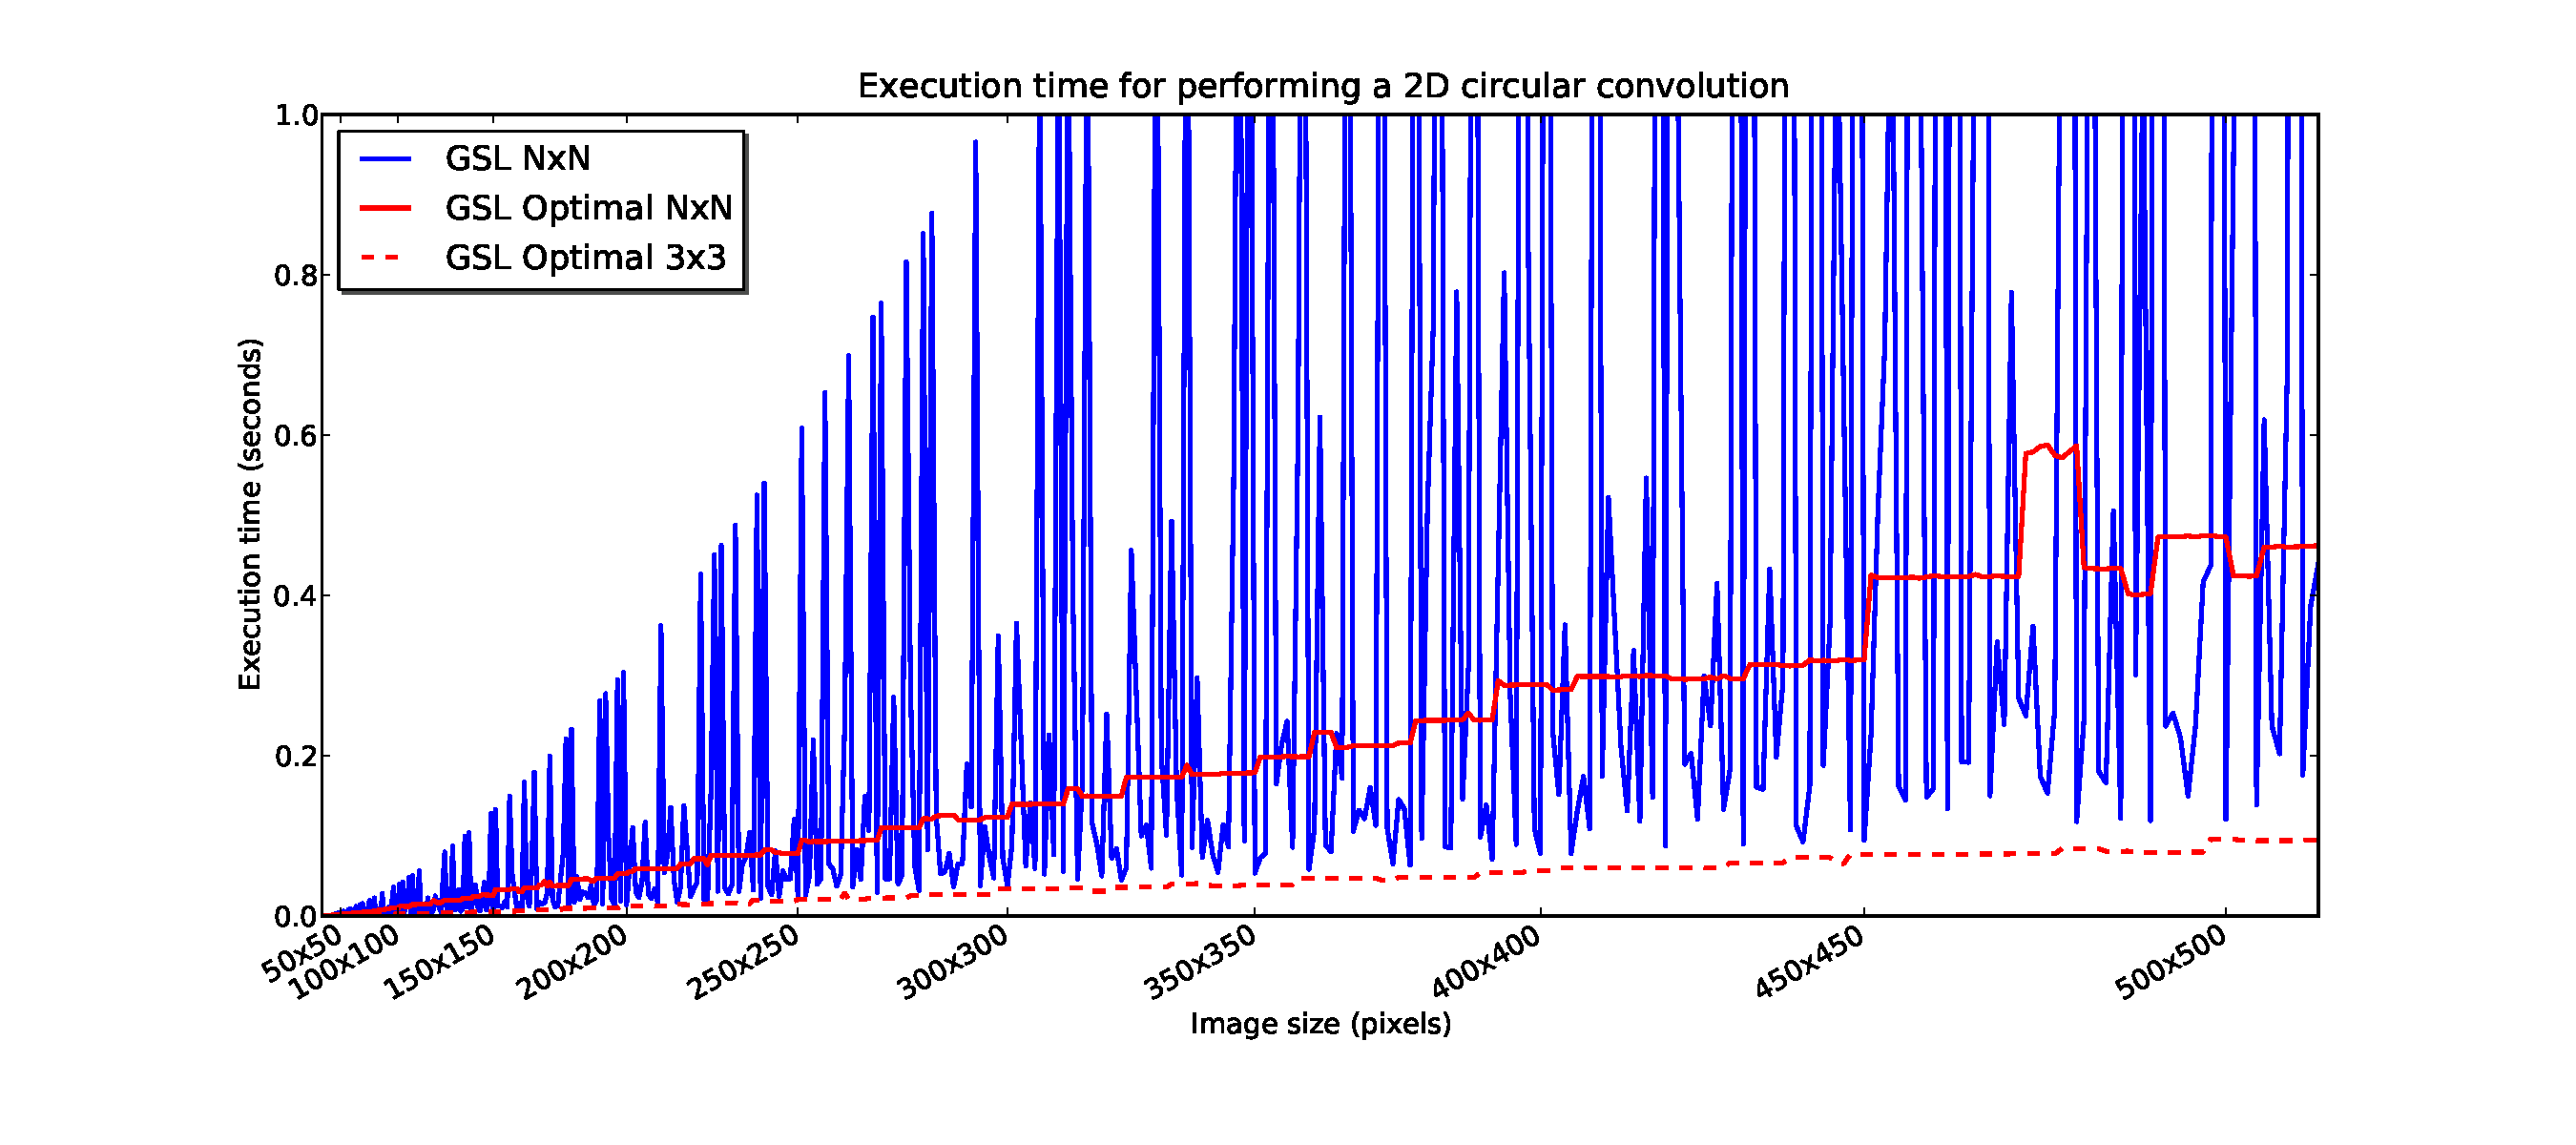
\includegraphics[width=0.75\linewidth]{../Images/benchmark_circular_convolution_gsl.pdf}
\caption{\label{fig:benchmark_circular_convolution_gsl.pdf}Execution time for performing a circular convolution with GSL. Two versions are plotted : with or without padding. The two curves of the padded version (solid and dashed) are the boundaries of the execution time, whatever the kernel size.}
\end{figure}

On the figure \ref{fig:benchmark_circular_convolution_fftw.pdf}, we see that there is no benefits in padding to get optimal sizes with FFTW. Circular convolution is what is computed by default when using the product of the FFTs. Therefore, when we pad an image to get optimal sizes but still to compute a circular convolution, we cannot be better than the non-padded version for optimal sizes and it depends for non-optimal sizes on the performance of the algorithm for these sizes. It appears that FFTW has rather good performances even for sizes it is not optimized for. This illustration was generated with the following script : \href{http://jeremy.fix.free.Fr/Software/Convolution/circular_convolution_fftw_benchmark.cc}{circular\_convolution\_fftw\_benchmark.cc}.\\

\begin{figure}[htbp]
\center 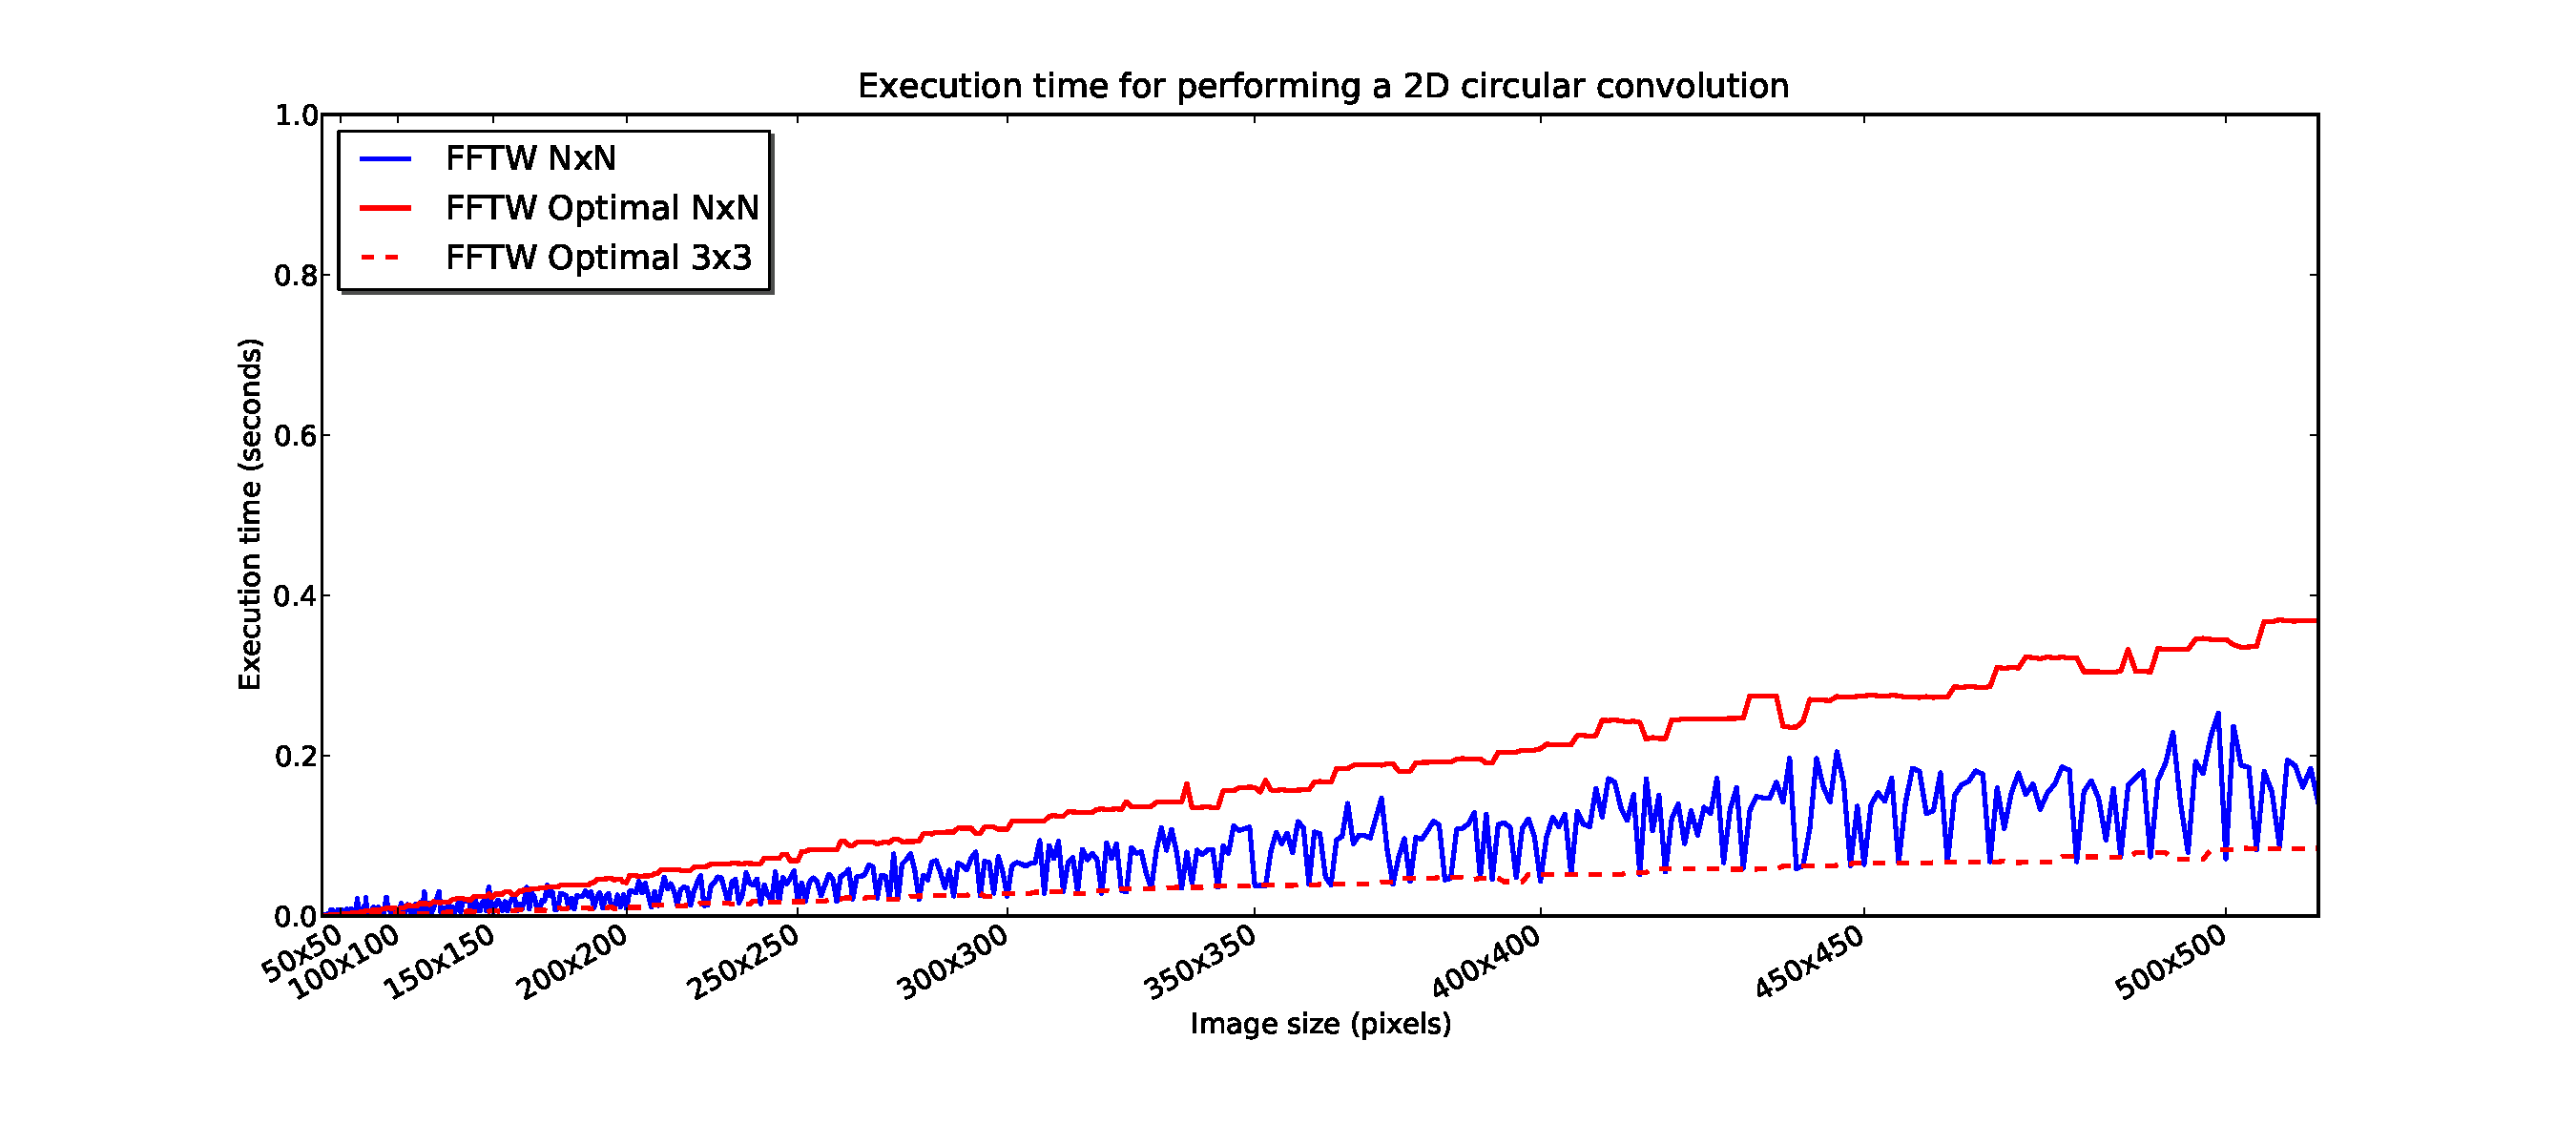
\includegraphics[width=0.75\linewidth]{../Images/benchmark_circular_convolution_fftw.pdf}
\caption{\label{fig:benchmark_circular_convolution_fftw.pdf}Execution time for performing a circular convolution with FFTW. Two versions are plotted : with and without padding with wrapped around values to get optimal sizes. For a circular convolution, padding makes the performances smoother but also worse !}
\end{figure}


To compare the execution times, we took the smallest execution time of the padded or unpadded convolution with the GSL, and the unpadded convolution of FFTW, and computed their ratio. The results are shown on figure \ref{fig:benchmark_circular_convolution_compare.pdf}. The FFTW based version appears to be better than the GSL based implementation. The differences are higher than for the linear convolution, with performances almost $75\%$ better, again for sizes at least $200 \times 200$.

\begin{figure}[htbp]
\center 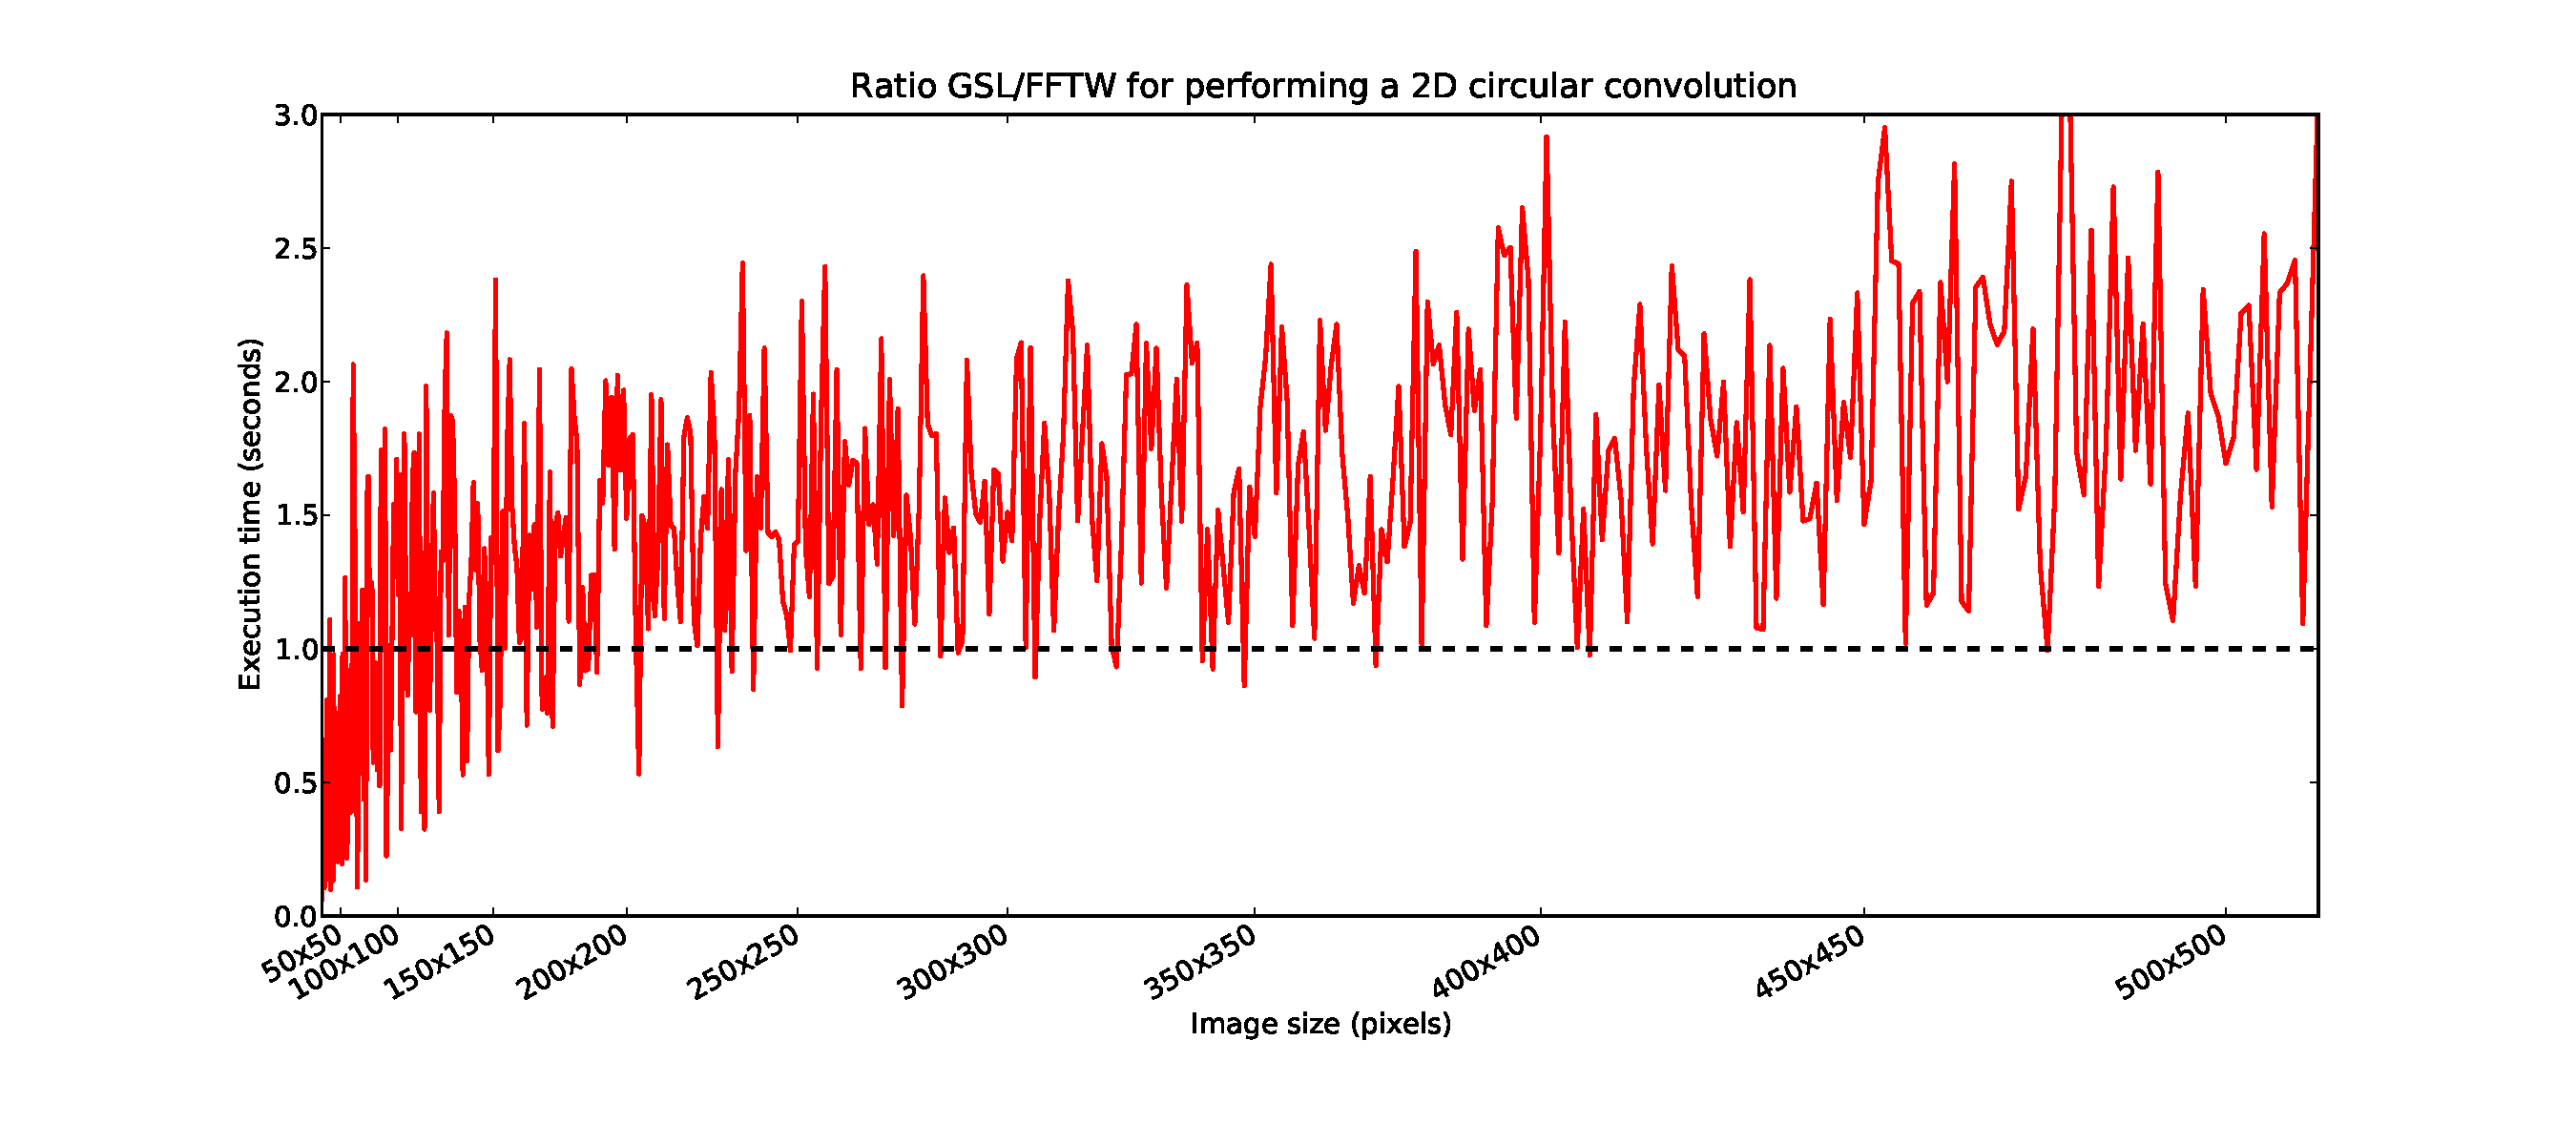
\includegraphics[width=0.75\linewidth]{../Images/benchmark_circular_convolution_compare.pdf}
\caption{\label{fig:benchmark_circular_convolution_compare.pdf} Comparison of the execution time for a circular convolution. For the GSL version, we used the minimum of the padded and unpadded times. For the FFTW version, we used the unpadded version. It seems that the FFTW version performs better.}
\end{figure}

\pagebreak
\subsection{Comparison between FFT based and standard convolution}

The previous benchmarks allowed to detect which FFT based algorithm was faster and if padding improves or not the performances. However, it is not always beneficial to use the FFT to compute a convolution product, simply because, with the FFT, you need to "resize" the kernel to the image size and compute the products of the two FFT. When convolving an image of size $N \times N$ with a kernel of size $K \times K$, you work with FFT of size $N \times N$ and compute pointwise products of images of size $N \times N$ which may cost more time than convolving with nested \emph{for loops}, especially if $K << N$.\\

To determine for which kernel size it is actually worth using the FFT, we ran again simulations of the FFT based convolution but now for different kernel sizes, to get a similar plot as the one for the standard convolution (fig. \ref{fig:benchmark_std_convolution.pdf}). We used the FFTW based implementation with the padded version for the linear convolution and the unpadded version for the circular convolution.


%We also saw that the performances depend on the kernel size. Here, we identify for which kernel sizes, it is actually worth using the FFT to compute a convolution compared to a standard convolution (with nested \emph{for loops}). On the figure \ref{fig:kernel_size.png}, we plot the kernel size $K$ for which convolving a $N\times N$ image with a kernel of size $K\times K$ ($K < N$) is always slower using a standard convolution than convolving a $N \times N$ image with a $N\times N$ kernel. From these benchmarks, it appears that it is for sure benefitial to use the FFT based convolution using FFTW to compute a 2D convolution when : 
%\begin{itemize}
%\item The kernel size is at least $18\times 18$ for a linear convolution
%\item The kernel size is at least $16\times 16$ for a circular convolution
%\end{itemize}
%
%\begin{figure}[htbp]
%\center 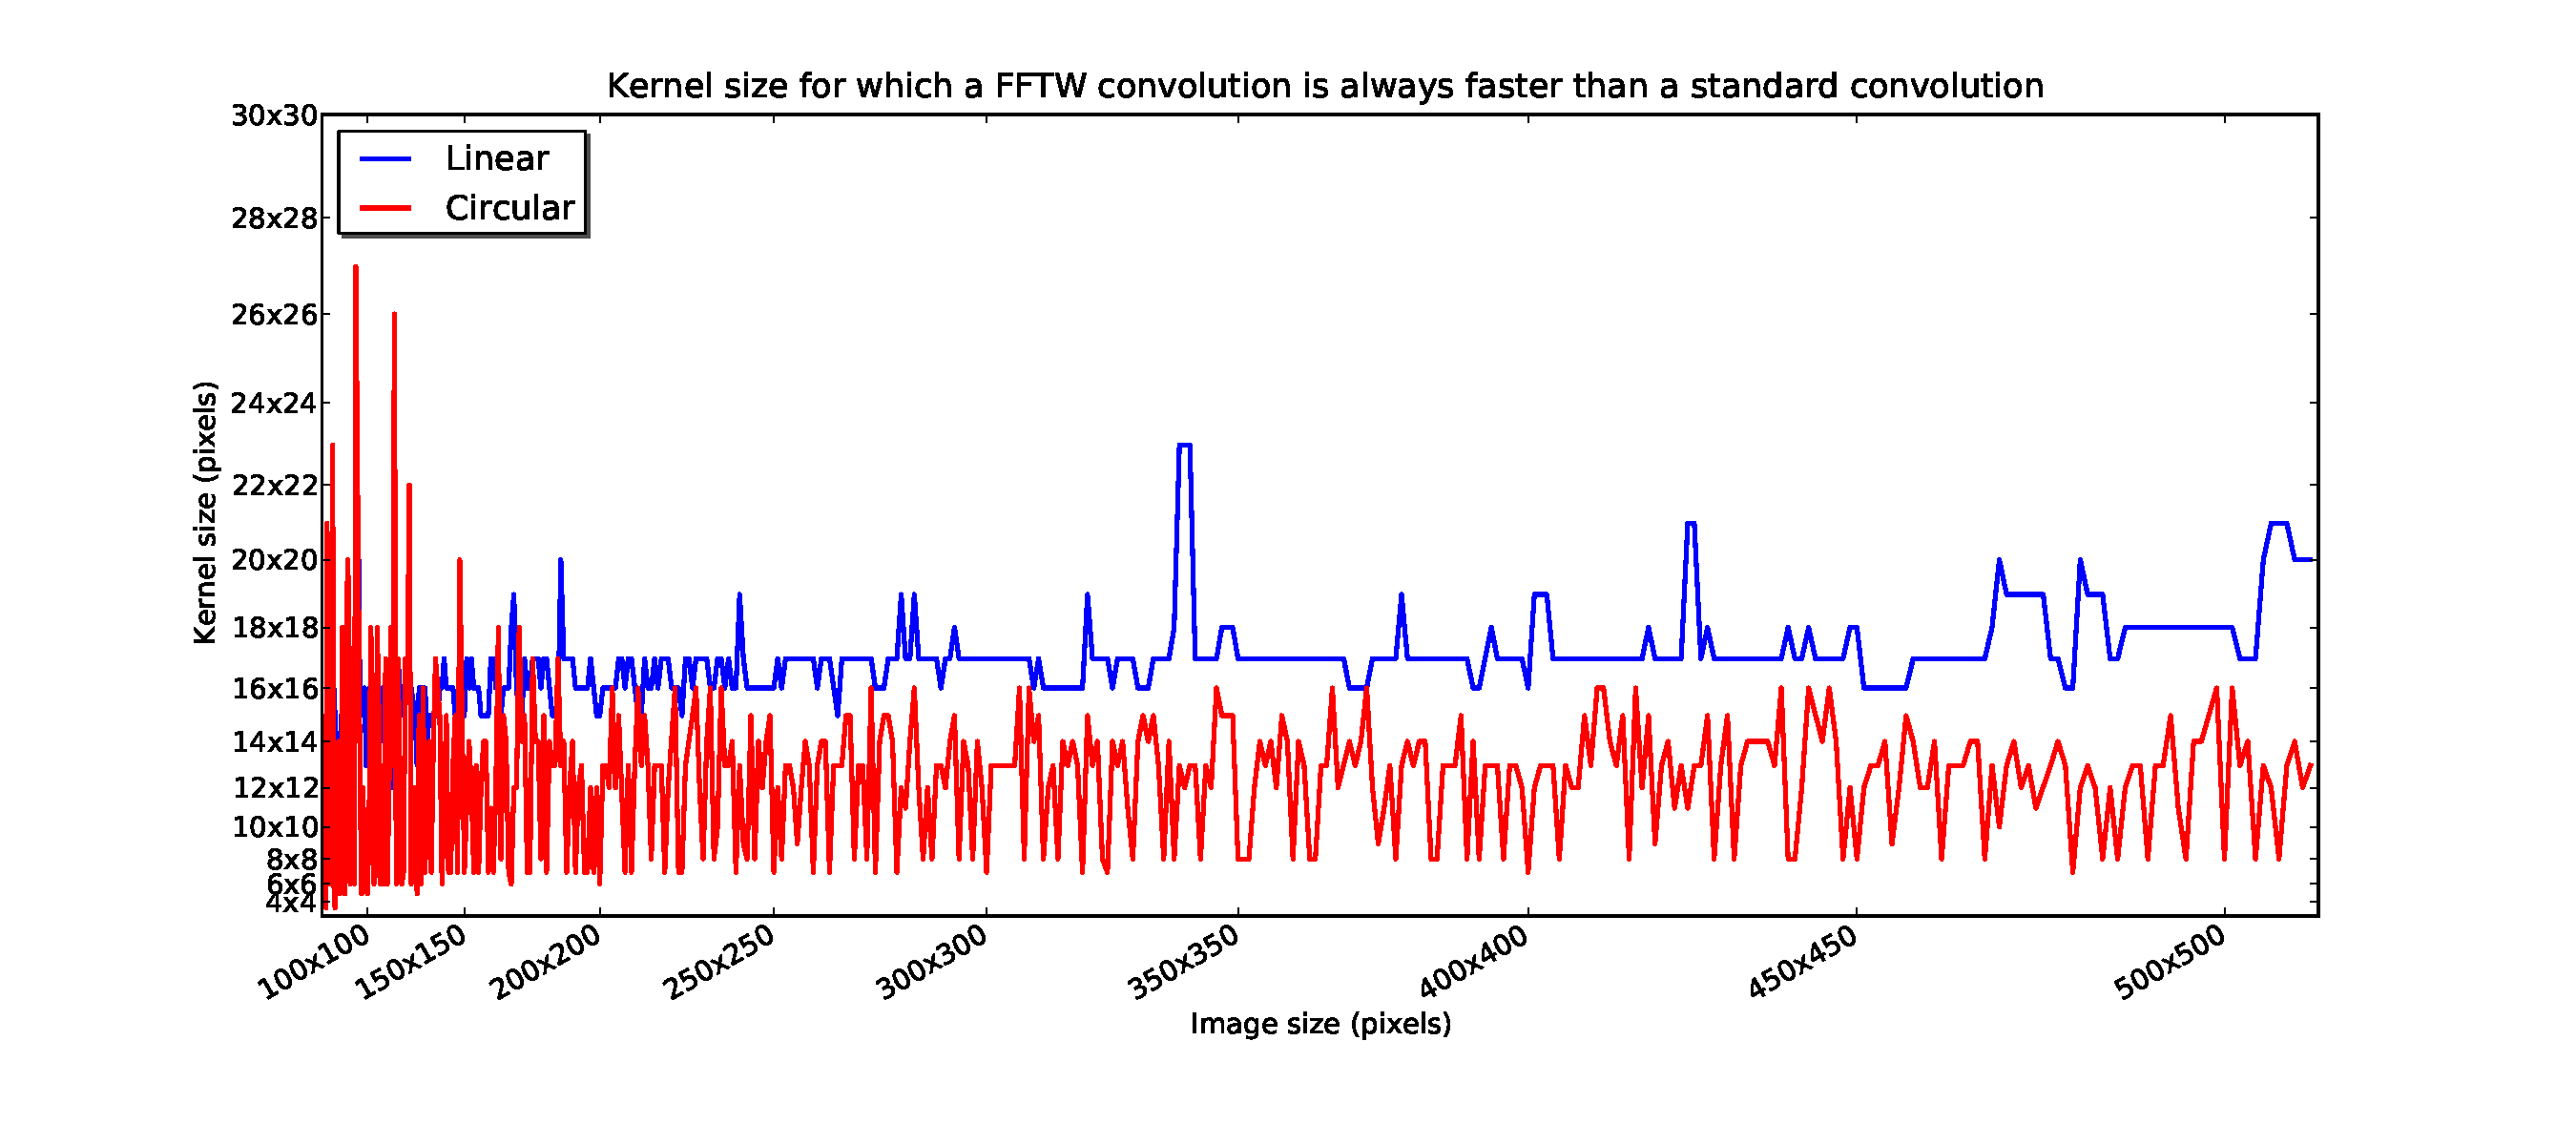
\includegraphics[width=.75\linewidth]{kernel_size.pdf}
%\caption{\label{fig:kernel_size.png} Minimal kernel size for which computing a convolution with the FFTW based implementation is faster than the nested for loops implementation, function of image size. The FFTW based implementation is faster than the nested for loops when the kernel is at least $18 \times 18$ for a linear convolution and $16\times 16$ for a circular convolution.}
%\end{figure}

\subsection{Putting everything together: 2D image Convolution using the FFT}

The scripts given in the previous section were using randomly generated matrices to perform the benchmarks. To process images, we make use of the \href{http://cimg.sourceforge.net/}{CImg library}. You just need to get the header CImg.h and put it at the same place of the script you compile. The scripts allowing to convolve an image with a filter are given below. These scripts compute 2 DFT at once (the source image and the kernel) and pad them with zeros or wrapped around pixel values to get optimal sizes.
\begin{itemize}
\item 2D Linear convolution with GSL : \href{http://jeremy.fix.Free.Fr/Software/Convolution/linear_convolution_gsl.cc}{linear\_convolution\_gsl.cc}
\item 2D Linear convolution with FFTW : \href{http://jeremy.fix.Free.Fr/Software/Convolution/linear_convolution_gsl.cc"}{linear\_convolution\_fftw.cc}
\item Circular convolution with GSL : \href{http://jeremy.fix.Free.Fr/Software/Convolution/circular_convolution_gsl.cc"}{circular\_convolution\_gsl.cc}
\item Circular convolution with FFTW : \href{http://jeremy.fix.Free.Fr/Software/Convolution/circular_convolution_gsl.cc"}{circular\_convolution\_fftw.cc}
\end{itemize}

On the figures \ref{fig:benchmark_linear_everything.pdf} and \ref{fig:benchmark_circular_everything.pdf} we compare the time it takes to compute a linear or circular convolution for different image and kernel sizes using FFTW, GSL and the nested for loops. In the previous sections, the benchmarks were always done with 2 images of the same size. This is rather unusual. Usually, the filter size is much smaller than the image size. To get an idea of how well the convolution involving the FFT performs, the execution time of a standard convolution (involving for loops) is also given. The illustrations were generated with the results of \href{http://jeremy.fix.Free.Fr/Software/Convolution/linear_everything.cc}{linear\_everything.cc} and \href{http://jeremy.fix.Free.Fr/Software/Convolution/circular_everything.cc}{circular\_everything.cc}.

\begin{figure}[htbp]
\center 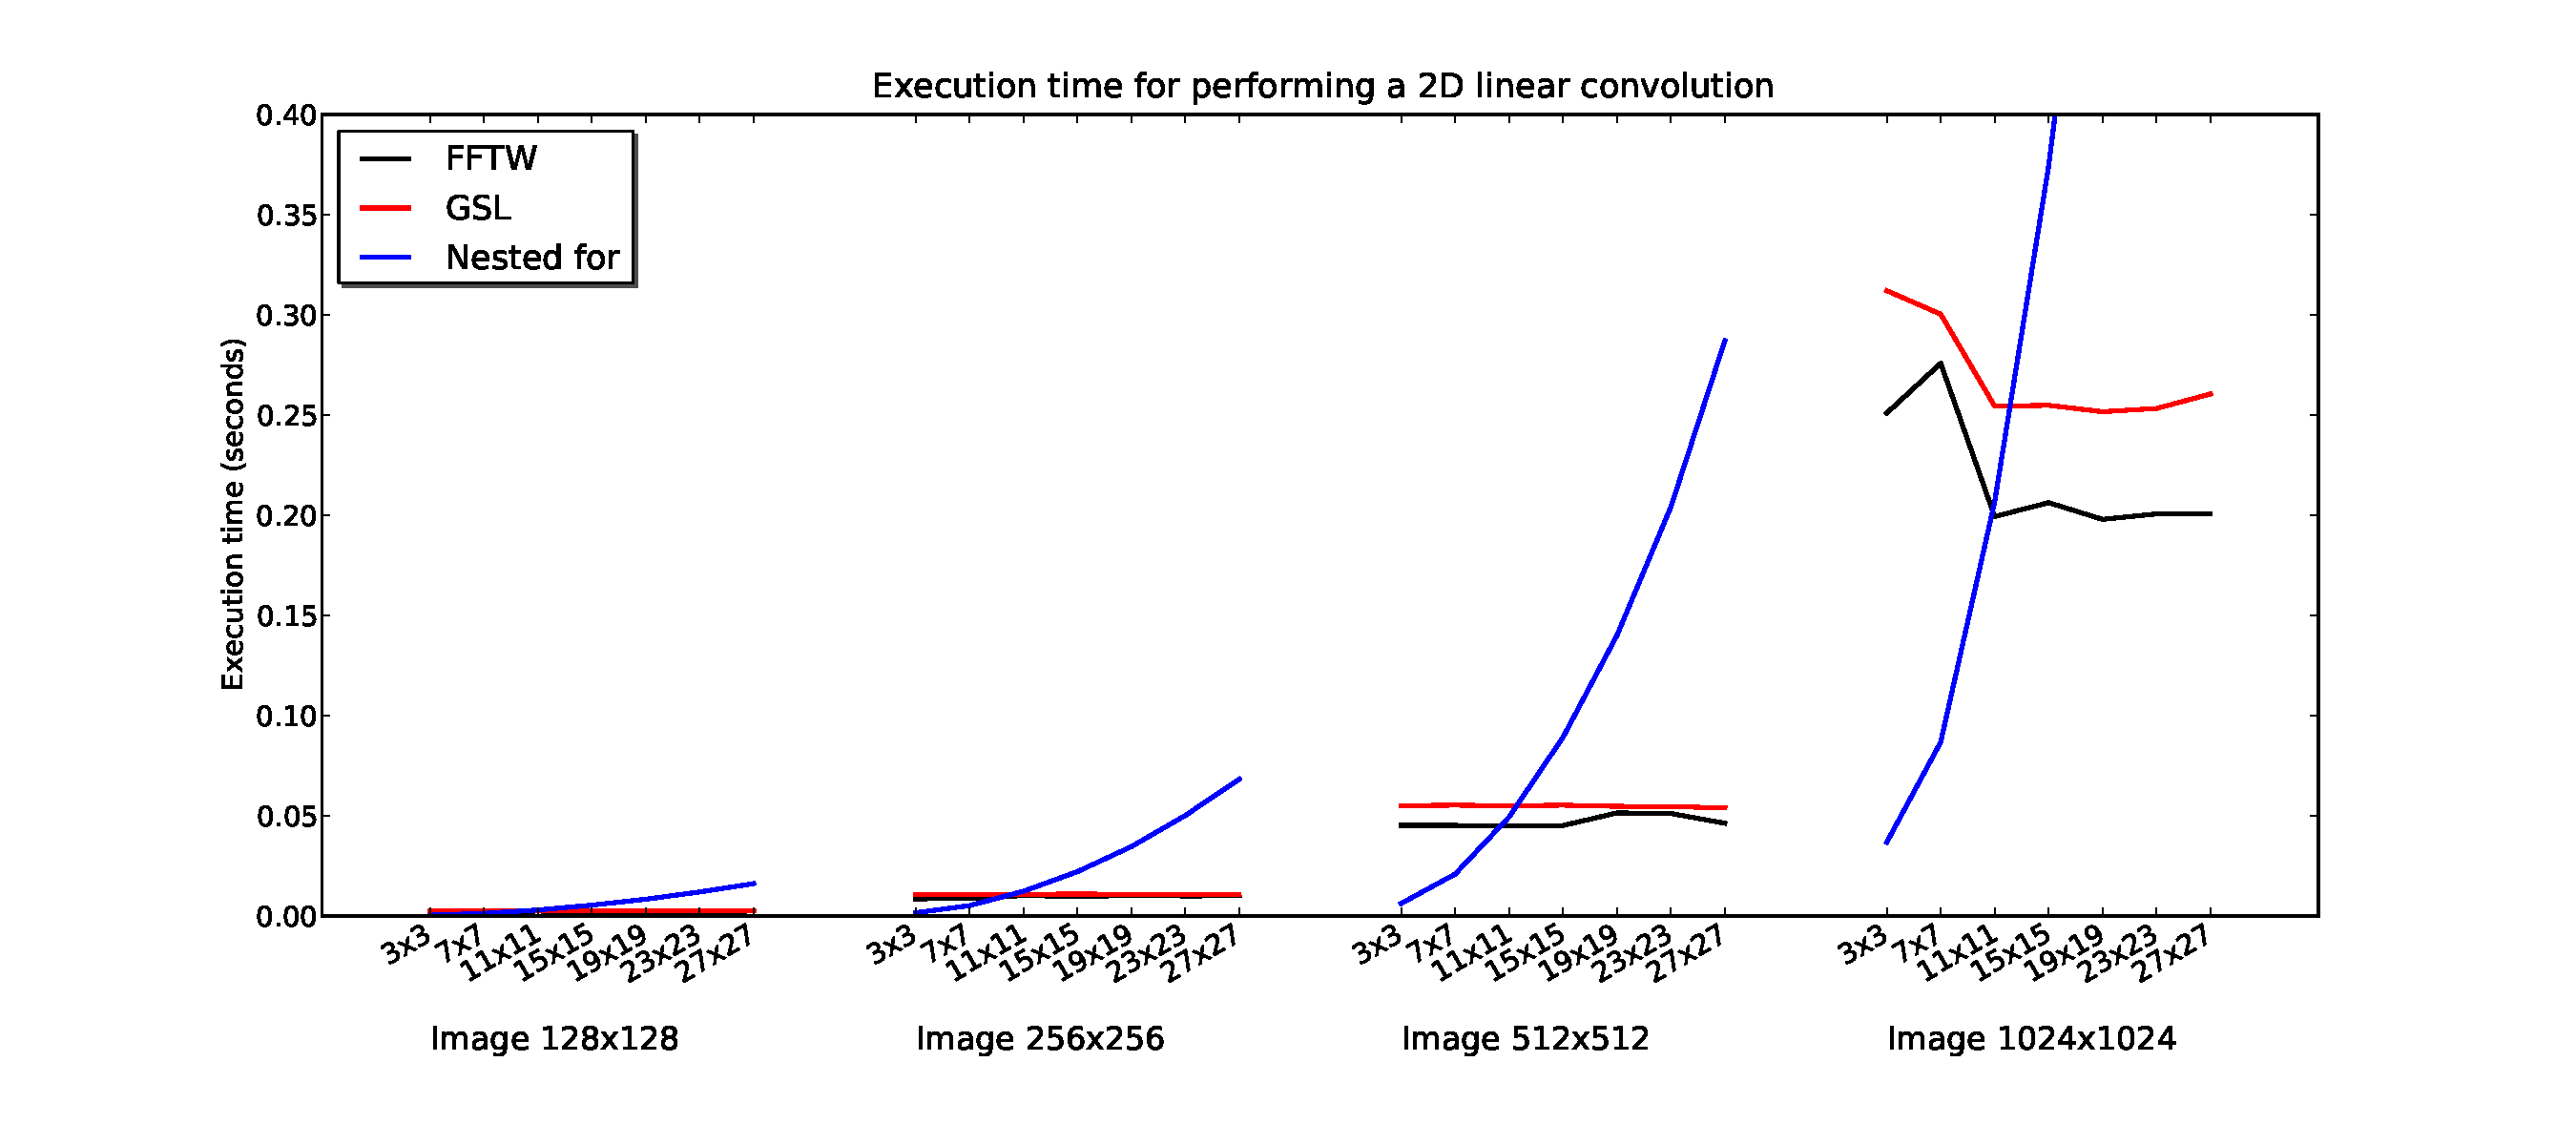
\includegraphics[width=.75\linewidth]{../Images/benchmark_linear_everything.pdf}
\caption{\label{fig:benchmark_linear_everything.pdf} Comparison of the processing time of a linear convolution with different image and filter sizes. Using a FFT based implementation is beneficial only above a certain filter size.}
\end{figure}

\begin{figure}[htbp]
\center 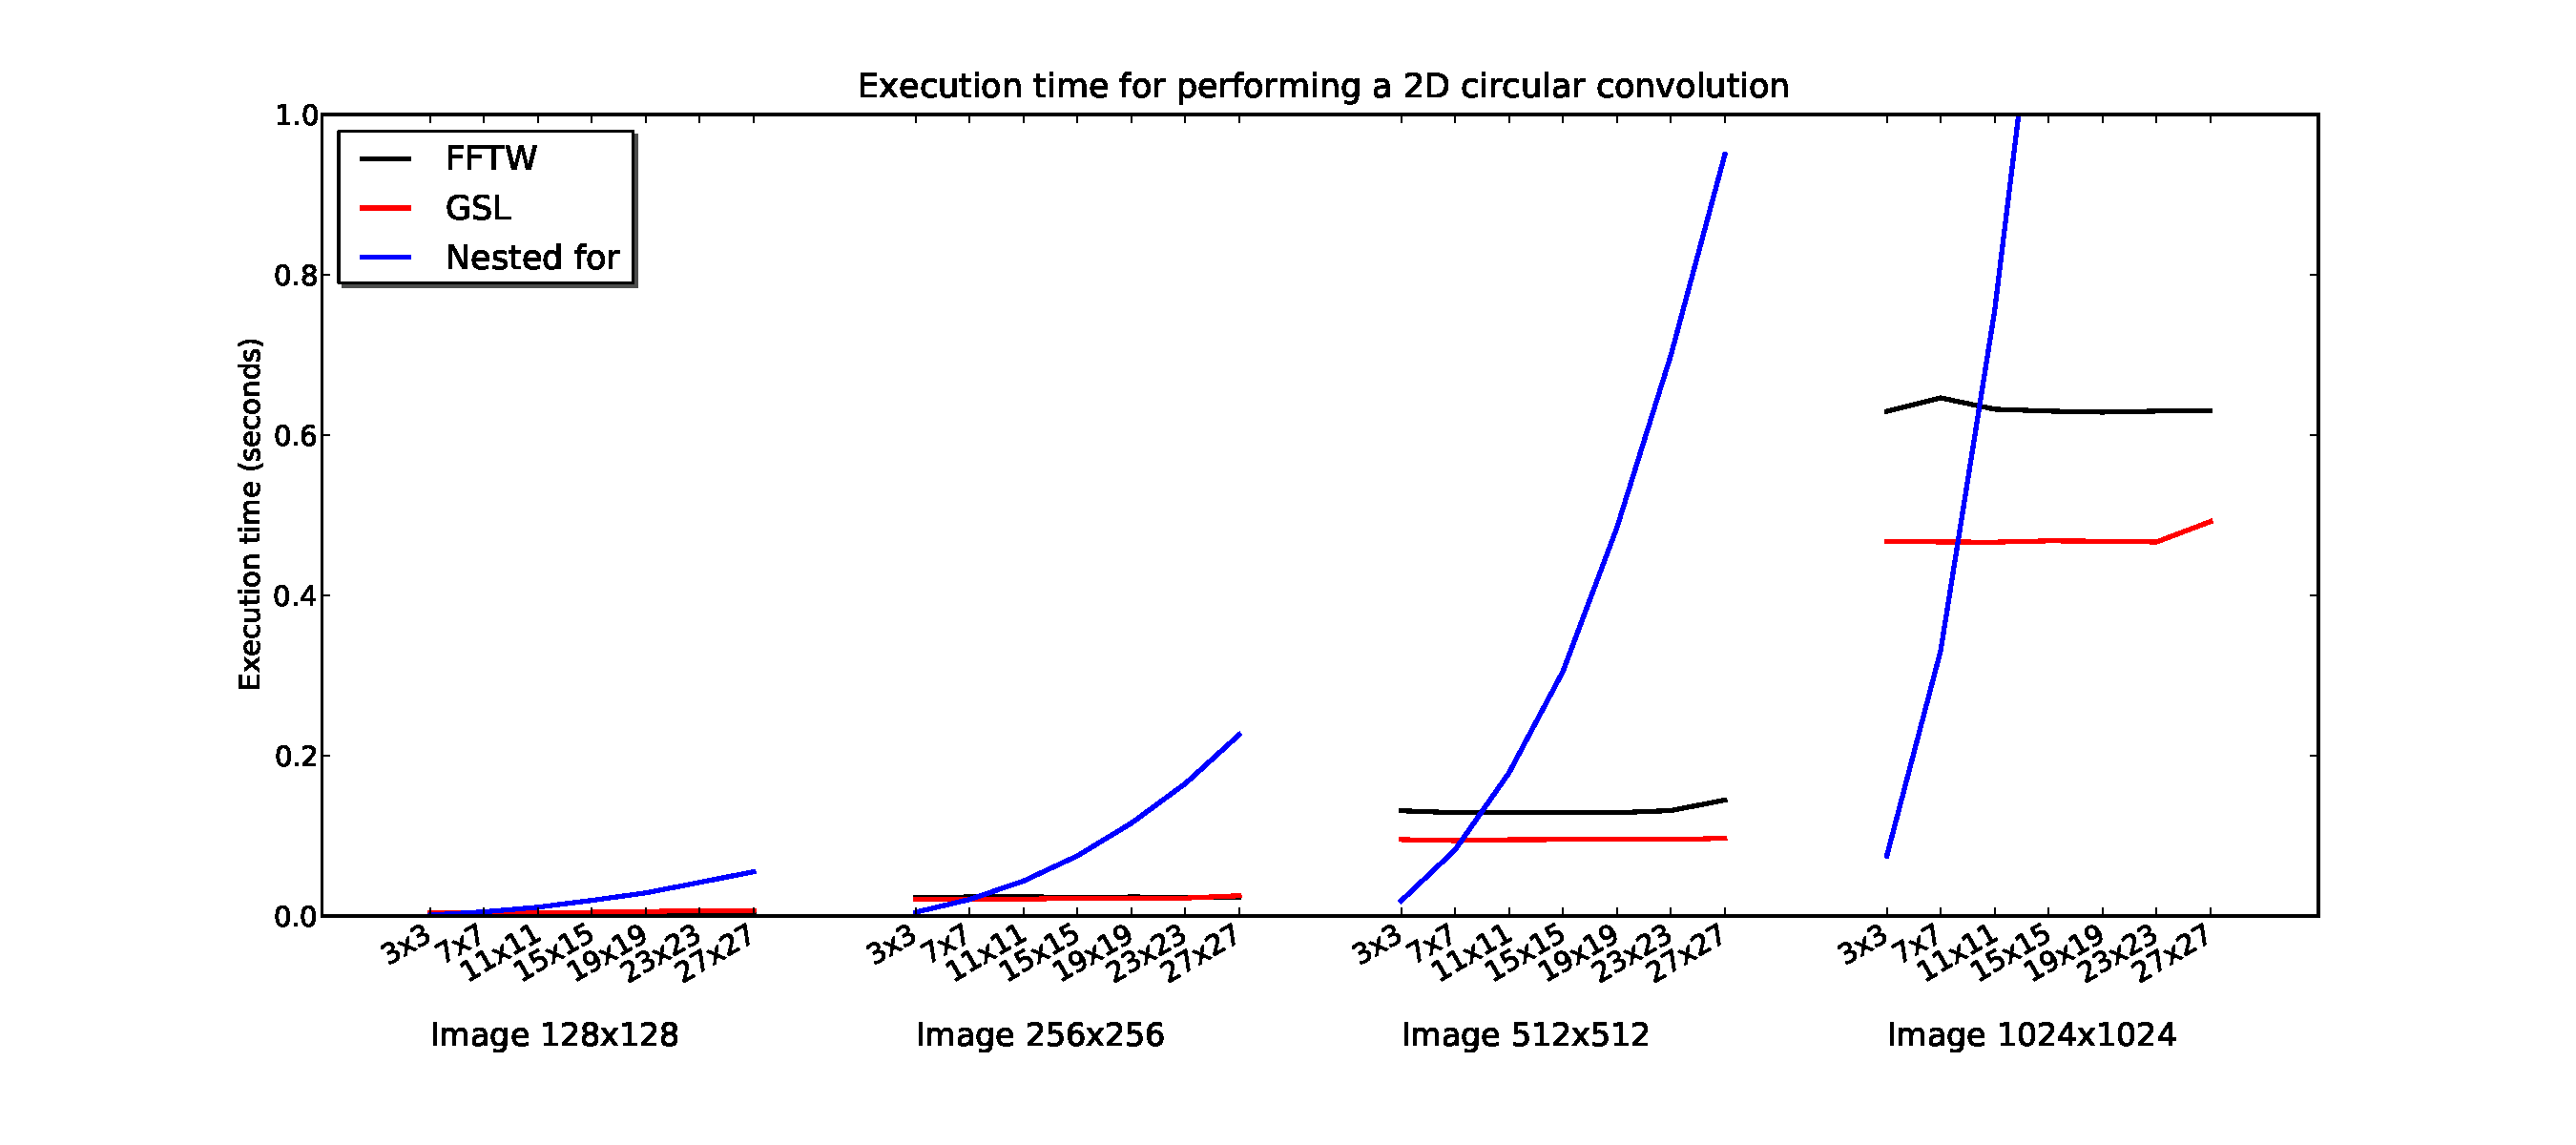
\includegraphics[width=.75\linewidth]{../Images/benchmark_circular_everything.pdf}
\caption{\label{fig:benchmark_circular_everything.pdf} Comparison of the processing time of a circular convolution with different image and filter sizes. Using a FFT based implementation is beneficial only above a certain filter size.}
\end{figure}

\section{C++ Implementations}

Here, we just provide a list of the C++ scripts used through this document :
\begin{itemize}
\item Computing a 2D Fourier Transform :
\begin{itemize}
\item with GSL : \href{http://jeremy.fix.Free.Fr/Software/Convolution/fft_gsl.cc}{fft\_gsl.cc}
\item with FFTW : \href{http://jeremy.fix.Free.Fr/Software/Convolution/fft_fftw.cc}{fft\_fftw.cc}
\end{itemize}
\item  Computing a linear convolution with nested for loops : \href{http://jeremy.fix.Free.Fr/Software/Convolution/std_convolution.cc}{std\_convolution.cc}
\item  Computing 2DFT at once with FFTW : \href{http://jeremy.fix.Free.Fr/Software/Convolution/2DFT.cpp}{2DFT.cpp}
\item  Computing a 2D linear convolution of randomly generated matrices with or without padding:
\begin{itemize}
\item with GSL : \href{http://jeremy.fix.Free.Fr/Software/Convolution/linear_convolution_gsl_benchmark.cc}{linear\_convolution\_gsl\_benchmark.cc}
\item with FFTW : \href{http://jeremy.fix.Free.Fr/Software/Convolution/linear_convolution_fftw_benchmark.cc}{linear\_convolution\_fftw\_benchmark.cc}
\end{itemize}
\item  Computing a 2D circular convolution of randomly generated matrices with or without padding:
\begin{itemize}
\item with GSL : \href{http://jeremy.fix.Free.Fr/Software/Convolution/circular_convolution_gsl_benchmark.cc}{circular\_convolution\_gsl\_benchmark.cc}
\item with FFTW : \href{http://jeremy.fix.Free.Fr/Software/Convolution/circular_convolution_fftw_benchmark.cc}{circular\_convolution\_fftw\_benchmark.cc}
\end{itemize}
\item  Computing a 2D linear convolution with images, using the optimal code :
\begin{itemize}
\item with GSL : \href{http://jeremy.fix.Free.Fr/Software/Convolution/linear_convolution_gsl.cc}{linear\_convolution\_gsl.cc}
\item with FFTW : \href{http://jeremy.fix.Free.Fr/Software/Convolution/linear_convolution_fftw.cc}{linear\_convolution\_fftw.cc}
\end{itemize}
\item  Computing a 2D circular convolution with images, using the optimal code :
\begin{itemize}
\item with GSL : \href{http://jeremy.fix.Free.Fr/Software/Convolution/circular_convolution_gsl.cc}{circular\_convolution\_gsl.cc}
\item with FFTW : \href{http://jeremy.fix.Free.Fr/Software/Convolution/circular_convolution_fftw.cc}{circular\_convolution\_fftw.cc}
\end{itemize}
\end{itemize}


\section{References}

\begin{itemize}
\item Discrete Fourier transform : definition and properties \href{http://en.wikipedia.org/wiki/Discrete_Fourier_transform}{link}
\item Convolution product : definition and properties \href{http://en.wikipedia.org/wiki/Convolution}{link}
\item Convolution theorem : \href{http://en.wikipedia.org/wiki/Convolution_theorem}{link}
\item Fast Fourier transform with the GSL : \href{http://www.gnu.org/software/gsl/manual/html_node/Fast-Fourier-Transforms.html}{link}
\item Fast Fourier transform with FFTW3 : \href{http://www.fftw.org/fftw3_doc}{link}
\item Book : Digital Signal Processing, J. Proakis, D. Manolakis. Chap 8 deals with computing 2 DFT at once : \href{http://www.amazon.com/Digital-Signal-Processing-John-Proakis/dp/0131873741}{link}
\end{itemize}


% --------------------    End     -------------------
\clearpage
\end{document}
